\documentclass[a4paper,12pt,amsmath,amssymb,aps]{article}
\usepackage[utf8]{inputenc}
\usepackage[danish]{babel}
\usepackage[T1]{fontenc}

% Fysik
\usepackage{physics}

% Matematik
\usepackage{amsmath,amssymb,bm,mathtools}
\usepackage{gensymb}
%\usepackage{breqn}
% Punktum i math-felter bliver til komma i pdf
%\DeclareMathSymbol{.}{\mathord}{letters}{"3B}

% SI-units
\usepackage[number-unit-product = \text{ }, inter-unit-product =\cdot]{siunitx}

% Figurer
\usepackage{graphicx}
\usepackage{float}

% Om dokumentet
\title{Dispositioner til AMO eksamen 6. juni 2019}
\author{Josefine Bjørndal Robl}
\date{\today}

% Marginer
\usepackage[tmargin=1.0in,bmargin=1in,lmargin=1.25in,rmargin=1.25in]{geometry}

% Header og footer
\usepackage{lastpage}
\usepackage{fancyhdr}
\pagestyle{fancy}
\lhead{
    Josefine Bjørndal Robl \\
	Aarhus Universitet - 201706760
}
\chead{}
\rhead{
	Atom- og Molekylfysik \\
	Eksamensdispositioner
}
\lfoot{}
\cfoot{}
\rfoot{Side \thepage\ af \pageref{LastPage}}
\renewcommand{\headrulewidth}{1pt}
\renewcommand{\footrulewidth}{1pt}

% Indryk tekst efter section og subsection
\usepackage{indentfirst}

% Ingen orddeling i section og subsection titler
\usepackage[raggedright]{titlesec}

% Ligninger nummereres 1.1, 1.2 osv. i section 1 og 2.1, 2.2 osv. i section 2
\numberwithin{equation}{section}

% Ligninger nummereres 1.1.1, 1.1.2 osv. i subsection 1 og 2.1.1, 2.1.2 osv. i subsection 2 - dog også 1.0.1 og 2.0.1 i hhv. section 1 og 2.
%\numberwithin{equation}{subsection}

% Subsections med uden at hedde f.eks. 0.1 og 0.2 (uden sections)
%\renewcommand{\thesubsection}{\arabic{subsection}}

% De angivne elementer nummereres 1.1, 1.2 osv. i section 1 og 2.1, 2.2 osv. i section 2
\usepackage{chngcntr}
\counterwithin{figure}{section}
\counterwithin{table}{section}

% Til at indsætte MATLAB kode i ShareLaTeX
% \usepackage{listings}
% \usepackage{color}
%     \definecolor{codegreen}{rgb}{0,0.6,0}
%     \definecolor{codegray}{rgb}{0.5,0.5,0.5}
%     \definecolor{codepurple}{rgb}{0.58,0,0.82}
%     \definecolor{backcolour}{rgb}{0.95,0.95,0.92}
% \lstdefinestyle{mystyle}{
%     backgroundcolor=\color{backcolour},
%     commentstyle=\color{codegreen},
%     keywordstyle=\color{magenta},
%     numberstyle=\tiny\color{codegray},
%     stringstyle=\color{codepurple},
%     basicstyle=\footnotesize,
%     breakatwhitespace=false,
%     breaklines=true,
%     captionpos=b,
%     keepspaces=true,
%     numbers=left,
%     numbersep=5pt,
%     showspaces=false,
%     showstringspaces=false,
%     showtabs=false,
%     tabsize=2
% }
% \lstset{style=mystyle}

% Lister med bindestreg som punkt
\renewcommand{\labelitemi}{\textendash}
\renewcommand{\labelitemii}{\textendash}
\renewcommand{\labelitemiii}{\textendash}
\renewcommand{\labelitemiv}{\textendash}

% Lister med bogstaver i stedet for tal
\usepackage{enumitem}
%\renewcommand{\theenumi}{\Alph{enumi}}

% Link/url - f.eks. så Table of content linker til section, subsection..., men også så url'er kan indsættes som clickable links.
\usepackage{hyperref}
\hypersetup{
    allcolors=black, % No colored links
    linktoc=all,     % "all" = both sections and subsections linked
}

% bra-ket notation
\usepackage{braket}
\renewcommand{\braket}{\Braket}

% Limit med limits under "lim"
\newcommand{\Lim}[2]{\raisebox{0.5ex}{\scalebox{0.8}{$\displaystyle \lim_{{#1} \rightarrow {#2}}\;$}}}
% Limit gående mod uendelig
\newcommand{\Liminf}[1]{\raisebox{0.5ex}{\scalebox{0.8}{$\displaystyle \lim_{{#1} \rightarrow \infty}\;$}}}
% Limit gående mod 0
\newcommand{\Limnul}[1]{\raisebox{0.5ex}{\scalebox{0.8}{$\displaystyle \lim_{{#1} \rightarrow 0}\;$}}}

% phi
\renewcommand{\phi}{\varphi}

% Til subfigures
\usepackage{caption}
\usepackage{subcaption}

% Pæne referencer med \cref
\usepackage{cleveref}
\crefname{equation}{ligning}{ligningerne}
\Crefname{equation}{Ligning}{Ligningerne}
\crefname{figure}{figur}{figurerne}
\Crefname{figure}{Figur}{Figurerne}
\crefname{table}{tabel}{tabellerne}
\Crefname{table}{Tabel}{Tabellerne}
\crefname{subsection}{underafsnit}{underafsnittene}
\Crefname{subsection}{Underafsnit}{Underafsnittene}
\crefname{section}{afsnit}{afsnittene}
\Crefname{section}{Afsnit}{Afsnittene}

\newcommand{\crefrangeconjunction}{ til } % Changes the ''to'' to <whatever is in the brackets'' when refering to a range of objects
\newcommand{\crefpairconjunction}{ og } % Changes the ''and'' to <whatever is in the brackets'' when refering to a pair of objects

% Fbjectsor sp of oacing between lines
\usepackage{setspace}
    % To change line spacing in the whole document use the command \linespread covered in Text Formatting.
    % Alternatively, you can use the \usepackage{setspace} package, which is also covered in Text Formatting. This package provides the commands \doublespacing, \onehalfspacing, \singlespacing and \setstretch{baselinestretch}, which will specify the line spacing for all sections and paragraphs until another command is used. Furthermore, the package provides the following environments in order to change line spacing within the document but not document-wide:
    %%% doublespace: lines are double spaced;
    %%% onehalfspace: line spacing set to one-and-half spacing;
    %%% singlespace: normal line spacing;
    %%% spacing: customizable line spacing, e.g. \begin{spacing}{\baselinestretch} ... \end{spacing}.

\usepackage[font={small,sl}]{caption}	% Caption med skrå tekst (ikke kursiv)


%%%%%%%%%%%%%%%%%%%%%%%%%%%%%%%%%%%%%%%%%%%%%%%%%%%%%%%%%%%%%%%%%%%%%%%%%%

\begin{document}

\maketitle

% Giver mulighed for sidehoved og -fod på titelsiden
\thispagestyle{fancy}

% SKRIV HERUNDER
\setcounter{tocdepth}{1}
\tableofcontents

\section[Bohrs atommodel]{Briefly outline Bohr's model of the atom. What are the main problems of this model?}

\noindent
\large
Sammenligning med solsystem grundet $F_\text{Coulomb} \propto 1/r^2$\\
Elektron i baner givet ved $F_\text{centripetal} = F_\text{Coulomb}$\\
Find udtryk for $\omega^2 = v^2/r^2$\\
Den totale energi i systemet\\
Postulater fra Bohr: Kvantiserede baner og energitab kun ved kvantespring\\
Problem I: Ingen stråling fra elektroner\\
Find radius fra antagelse om kvantiseret impulsmoment\\
Bohrs formel
\begin{itemize}
    \item Bølgetal ved Bohrs formel sammenlignet med bølgetal fra Rydbergs formel
    \item Rydbergkonstanter stemmer stort set overens men\ldots
\end{itemize}
Problem II: Antagelse om uendelig tung kerne
\begin{itemize}
    \item Løsning ved reduceret masse i stedet for \ldots
    \item Isotropskift
\end{itemize}
Problem III: Mangel på spin
\begin{itemize}
    \item \ldots
\end{itemize}
\normalsize
\subsection{Briefly outline Bohr's model of the atom. What are the main problems of this model?}

Bohrs atommodel bygger på den kendte viden fra Rutherfords eksperiment om, at atomer består af en lille og tung kerne med positiv ladning. Ser vi på hydrogen har vi en proton som kerne og en elektron kredsende omkring denne. Tiltrækningen mellem de to ladede partikler er givet ved Couloubkraften, hvilken er invers proportional med $r^2$ ligesom tyngdekraften er, hvorfor Bohrs atommodel bygger på den klassiske model for et tolegmesystem, f.eks. en planet omkring en stjerne, hvor banen er en cirkelbane, som fra klassiske mekanik opretholdes af en balance mellem centripetalkraften og Coulombbkraften
\begin{align} \label{eq:Q01_Centripetalkraft=Coulombkraft}
	\frac{m_e v^2}{r} &= F_\text{centripetal} = F_\text{Coulomb} = \frac{e^2}{4\pi\epsilon_0 r^2} \: ,
\end{align}
hvor $m_e$ er elektronens masse, $v$ er elektronens fart, $e$ er elementarladningen, hvilken er svarende til størrelsen af ladningen af en elektron eller proton, og $r$ er radius af banen.

Fra dette kan vinkelfrekvensen $\omega = v/r$ bestemmes
\begin{align}
    \frac{1}{r}\frac{m_e v^2}{r} &= \frac{m_e v^2}{r^2} = \frac{1}{r}\frac{e^2}{4\pi\epsilon_0 r^2} = \frac{e^2}{4\pi\epsilon_0 r^3} \nonumber\\
    \Rightarrow \omega^2 &= \frac{v^2}{r^2} = \frac{e^2}{4\pi\epsilon_0 m_e r^3} \: ,
\end{align}
hvilket er ækvivalent til Keplers lov, hvilket også var formodet, da der er benyttet de samme antagelser og atomet lige pt. er beskrevet fuldstændig klassisk.

Den totale energi i en sådan banebevægelse er givet ved summen af den kinetiske og potentielle energi
\begin{align}
    E &= T - U = \frac{1}{2}m_e v^2 - \frac{e^2}{4\pi\epsilon_0 r} \: ,
\end{align}
og ved at benytte \cref{eq:Q01_Centripetalkraft=Coulombkraft} fås den kinetiske energi til at være halvdelen af den potentielle energi
\begin{align}
    m_e v^2 &= \frac{e^2}{4\pi\epsilon_0 r^2}r = \frac{e^2}{4\pi\epsilon_0 r} \: ,
\end{align}
så den totale energi bliver
\begin{align} \label{eq:Q01_TotalenergiIHydrogenAtom}
    E &= - \frac{1}{2}\frac{e^2}{4\pi\epsilon_0 r} = - \frac{e^2}{8\pi\epsilon_0 r} \: ,
\end{align}
hvilken er negativ, da elektronen er i en bunden banebevægelse, så der skal tilføres energi til systemet for at fjerne elektronen fra banen.

Bohr formodede da, at kun baner med bestemte energier var tilladte, og at elektronen kun ændrer energi, når den hopper mellem baner, og denne overskudsenergi, når den hopper fra en yderlige bane til en inderligere bane, udsendes som lys af en bølgelængde bestemt ved energiforskellen mellem banerne.

\paragraph{Problem I -- Ingen stråling:} Bohr antager, at en ændring af energi kun kan finde sted, når elektronen hopper mellem de tilladte baner, men ud fra klassisk elektrodynamik udsender en accelererende ladet partikel energi i form af elektromagnetiske bølger (lys), men dette ville også betyde, at elektronen gradvist ville spiralere ind mod protonen og dermed også kunne forholde sig i mellemrummet mellem de tilladte baner. Dette stemmer ikke overens med Bohrs andre antagelser, hvorfor han antog -- da modellen ikke forklarer det -- at elektronen ikke radierer i dens banebevægelse, hvilket viser sig at holde stik med de eksperimentelle data.

Bohr postulerede, at impulsmomentet var kvantiseret,
\begin{align}
    m_e v r &= n\hbar \: , \quad \forall n\in \mathbb{N} \: ,
\end{align}
hvorfor energien ville blive kvantiseret.
Kombineres denne med \cref{eq:Q01_Centripetalkraft=Coulombkraft} fås radius som værende
\begin{align} \label{eq:Q01_RadiusSomFunktionAfN}
    \frac{m_e v^2}{r} &= \frac{e^2}{4\pi\epsilon_0 r^2} \nonumber\\
    \Rightarrow \frac{1}{r} &= \frac{e^2}{4\pi\epsilon_0 m_e v^2 r^2} = \frac{e^2 m_e}{4\pi\epsilon_0 m_e^2 v^2 r^2} \nonumber\\
    \Rightarrow r &= \frac{4\pi\epsilon_0 m_e^2 v^2 r^2}{e^2 m_e} = \frac{4\pi\epsilon_0 \hbar^2 n^2}{e^2 m_e} = \frac{\hbar^2 n^2}{\left(e^2/4\pi\epsilon_0\right) m_e} = a_0 n^2 \: ,
\end{align}
hvor $a_0$ er Bohrradien,
\begin{align}
    a_0 &= \frac{\hbar^2}{\left(e^2/4\pi\epsilon_0\right) m_e} \: .
\end{align}
Fra \cref{eq:Q01_TotalenergiIHydrogenAtom} og \cref{eq:Q01_RadiusSomFunktionAfN} kan man få Bohr formlen
\begin{align} \label{eq:Q01_BohrsFormel}
    E &= - \frac{e^2}{8\pi\epsilon_0 r} = - \frac{e^2}{8\pi\epsilon_0 a_0} \frac{1}{n^2} \: ,
\end{align}
hvor $n$ kaldes \textsf{hovedkvantetallet} (eng. principal quantum number).
Bohrs formel forudsiger, at lyset udsendt fra overgange, $n' \rightarrow n$, mellem de tilladte baner i atomet vil have bølgetal ($\tilde{\nu} = 1/\lambda$)
\begin{align} \label{eq:Q01_BoelgetalFraBohrsFormel}
    \tilde{\nu} &= R_\infty \left(\frac{1}{n^2} - \frac{1}{n'^2}\right) \: .
\end{align}
Udregnes de mulige bølgetal for hydrogen vil disse stemme forholdsvis overens med de udregnede bølgetal fra Rydbergs formel,
\begin{align}
    \tilde{\nu} &= \frac{1}{\lambda} = R \left(\frac{1}{n^2} - \frac{1}{n'^2}\right) \: .
\end{align}
Rydbergkonstanten $R_\infty$ i \cref{eq:Q01_BoelgetalFraBohrsFormel} er defineret som
\begin{align}
    hcR_\infty &= \frac{\left(e^2/4\pi\epsilon_0\right)^2 m_e}{2\hbar^2} \: ,
\end{align}
hvor $hc$ er en konversionsfaktor mellem energi og kvantetal, siden $R_\infty$ er givet i enheder af $\si{\per\metre}$ (eller $\si{\per\centi\metre}$, hvilket normalt benyttes). I laboratoriet har man ved hjælp af lasere kunnet finde en utrolig præcis værdi for Rydbergkonstanten $R_\infty = \SI{10973731.568525}{\per\metre}$.

\paragraph{Problem II -- Antagelse om uendelig tung kerne:} Selvom Bohrs formel giver en Rydbergkonstant $R_\infty$ meget tæt på værdien af Rydbergkonstanten for et hydrogenatom $R_H$, så er der et problem med den, hvilket kommer af, at Bohr har antaget en fikseret kerne, altså en uendelig tung kerne (hvorfor det nedsænkede $\infty$). I realiteten bevæger både protonen og elektronen rundt om deres samlede massemidtpunkt (center of mass). For en kerne med en endelig masse $M$, da kan ligningerne modificeres ved at udskifte elektronens masse $m_e$ med den reducerede masse
\begin{align}
    m &= \frac{m_e M}{m_e + M} \: ,
\end{align}
hvilket for hydrogen giver Rydbergkonstanten
\begin{align}
    R_H &= R_\infty \frac{M_p}{m_e + M_p} \simeq R_\infty \left(1 - \frac{m_e}{M_p}\right) \: ,
\end{align}
hvor elektronmasse-til-protonmasse-forholdet er $m_e/M_p \simeq 1/1836$. Dette forhold er forskelligt for isotoperne af et grundstof, f.eks. hydrogen og deuterium, hvilket giver små men observerbare forskelle i frekvensen af det udsendte lys for forskellige isotoper af et grundstof, hvilket kaldes isotopskift.


\paragraph{Problem III:} Mangel på spin, og dermed fin- og hyperfinstruktur. Mangel på relativistiske effekter. \ldots

\section[Atom-lysvekselvirkning og Einsteinkoefficienter]{Describe interaction of atoms with light by using the Einstein coefficients. Establish relationships between these coefficients. Relate the Einstein coefficients to spectroscopic experiments.}

\noindent
\Large

\normalsize
\subsection{Describe interaction of atoms with light by using the Einstein coefficients. Establish relationships between these coefficients. Relate the Einstein coefficients to spectroscopic experiments.}


\begin{figure}[!h]
    \centering
    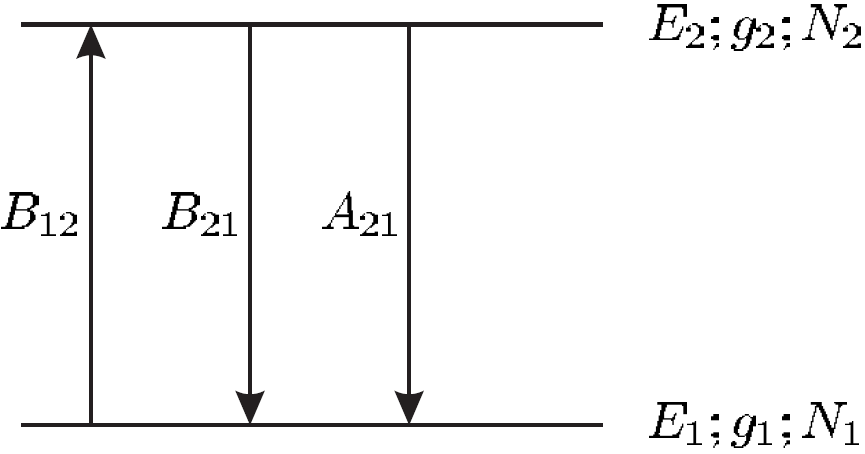
\includegraphics[width=0.5\textwidth]{Q02/images/TwoLevelSystem2.PNG}
    \caption{Toniveausystem med energier $E_1$ og $E_2$, som kan være udarter med $g_1$ og $g_2$, samt har en startpopulation på $N_1$ og $N_2$. Einsteinkoefficienterne $B_{12}$, $B_{21}$ og $A_{21}$ angiver hhv. (stimuleret) absorption, stimuleret emission og spontan emission.}
    \label{fig:Q02_TwoLevelSystem}
\end{figure}

Vi betragter et toniveausystem med energier $E_1$ og $E_2$ i hhv. tilstand $\ket{1}$ og $\ket{2}$. Energiniveauerne har en udartethed (eng. degeneracy) på hhv. $g_1$ og $g_2$, og niveauerne starter med at indeholde hhv. $N_1$ og $N_2$ atomer. Vi sender lys med enrgitæthed $\rho(\omega)$ per frekvensenhed ind på vores toniveausystem, hvilket skaber overgange fra $\ket{1}$ til $\ket{2}$ med en rate, der er proportional med $\rho(\omega_{12})$, hvor proportionalitetskonstanten er $B_{12}$. Atomet interagerer kun med den del af energifordelingen $\rho(\omega)$, som har en frekvens tæt på atomets \textsf{resonansfrekvens} $\omega_{12} = (E_1 - E_2)/\hbar$. Per symmetri vil det også formodes, at lyset vil skabe overgange fra $\ket{2}$ til $\ket{1}$ med en rate, der stadig er proportionel med $\rho(\omega)$, men har proportionalitetskonstant $B_{21}$. Førstnævnte er et tilfælde af (stimuleret) absorption, mens sidstnævnte er et tilfælde af stimuleret emission, hvor lyset med vinkelfrekvens $\omega$ vil få atomet til at udsende lys med denne samme frekvens.\footnote{This increase in the amount of light at the incident frequency is findaental to the operation of lasers. The word \textsf{laser} is an acronym for Light Amplification by Stimulated Emission of Radiation.} Denne symmetri mellem stimuleret absorption og emission bliver dog ødelagt af spontan emission, hvor en elektron falder ned til det laveste energiniveau ($\ket{2} \rightarrow \ket{1}$) selvom den ikke er blevet belyst. Raten af denne spontane emission beskrives ved $A_{21}$.

\underline{Opsummeret:} Bliver et atom ramt af lys med frekvens $\omega$ tæt på atomets resonsfrekvens $\omega_{12} = \Delta E / \hbar$ vil der ske en ændring af populationen i energiniveauerne ved en af følgende muligheder, beskrevet ved de givne Einsteinkoefficienter:
\begin{itemize}
    \item $B_{12}$: \textbf{Absorption} af en foton exciterer en elektron fra $\ket{1}$ til $\ket{2}$.
    \item $B_{21}$: Absorption af en foton vil (per symmetri) udløse en \textbf{stimuleret emission} af en foton af samme frekvens som den indkomne, samt lade en elektron falde fra $\ket{2}$ ned til $\ket{1}$.
    \item $A_{21}$: Uden at blive ramt af de indkomne fotoner kan der forekommer \textbf{spontan emission}, hvilket udsender en foton med atomets resonsnsfrekvens og derved bringe en elektron fra $\ket{2}$ til $\ket{1}$. Dette forekommer med en rate (eng. decay rate) på $A_{21} = 1/\tau$, hvor $\tau^{-1}$ er den gennemsnitlige levetid for $\ket{2}$.
\end{itemize}

Rateligningerne (eng. the rate equations) for populationerne $N_1$ og $N_2$ for tilstandene $\ket{1}$ og $\ket{2}$ bliver derved
\begin{align}
    \frac{\text{d}N_2}{\text{d}t} &= N_1 B_{12} \rho(\omega_{12}) - N_2 B_{21} \rho(\omega_{12}) - N_2 A_{21} \: , \quad \text{og} \label{eq:Q02_RateEquationN2}\\
    \frac{\text{d}N_1}{\text{d}t} &= - \frac{\text{d}N_2}{\text{d}t} \: , \label{eq:Q02_RateEquationN1} \: .
\end{align}
\Cref{eq:Q02_RateEquationN2} giver ændringsraten for $N_2$ som funktion af hhv. absorption, stimuleret emission og spontal emission, mens \cref{eq:Q02_RateEquationN1} er en konsekvens af, at der kun er to energiniveauer, så elektronerne, som forlader $\ket{2}$, må komme til $\ket{1}$.

Idet at der intet lys er ($\rho(\omega) = 0$), og der befinder sig elektroner i $\ket{2}$ ($N_2(0) \ne 0$), så vil ligningerne få en eksponentielt aftagende løsning
\begin{align}
    N_2(t) &= N_2(0)\exp{-A_{21}t} = N_2(0)\exp{-\frac{t}{\tau}} \: ,
\end{align}
hvor $\tau$ er den gennemsnitlige levetid.


\paragraph{Sammenhæng mellem A og B koefficienterne:} For at finde sammenhængen mellem Einsteinkoefficienterne betragtes det føromtalte atom (toniveausystem) beliggende i et område af sortlegemestråling (eng. black-body radiation). Her vil energitætheden $\rho(\omega)\,\text{d}\omega$ i vinkelfrekvensintervallet $[\omega,\: \omega + \text{d}\omega]$ kun afhænge af temperaturen $T$ af sortlegemet. Dette er givet af Plancks lov
\begin{align} \label{eq:Q02_PlancksLov}
    \rho(\omega) &= \frac{\hbar\omega}{\pi^2c^3} \dfrac{1}{\exp{\dfrac{\hbar\omega}{k_B T}} - 1} \: .
\end{align}
Betragtes nu på populationerne, når der er ligevægt (eng. equilibrium), $\frac{\text{d}N_2}{\text{d}t} = 0$, så populationerne ikke ændrer sig, så kan 
\begin{align} \label{eq:Q02_rho(omega)ILigevaegt}
    0 &= N_1 B_{12} \rho(\omega_{12}) - N_2 B_{21} \rho(\omega_{12}) - N_2 A_{21} \nonumber\\
    N_2 A_{21} &= \left(N_1 B_{12} - N_2 B_{21}\right) \rho(\omega_{12}) \nonumber\\
    \Rightarrow \rho(\omega_{12}) &= \frac{A_{21}}{B_{21}} \dfrac{1}{\dfrac{N_1 B_{12}}{N_2 N_{21}} - 1} \: .
\end{align}
I termisk ligevægt vides det, at populationerne i hvert af tilstandene\footnote{Der er $g_i$ udartede tilstande i ét energiniveau $E_i$}, som er i energiniveauerne, vil være givet ved Boltzmannfaktoren, og populationen i hver af tilstandene er giver som populationen i energiniveauet delt med antallet af udartede tilstande i niveauet, hvorfor
\begin{align} \label{eq:Q02_VedBrugAfTermiskLigevaetOgBoltzmannfaktoren}
    \frac{N_2}{g_2} &= \frac{N_1}{g_1}\exp{-\frac{\hbar\omega}{k_B T}} \: .
\end{align}

Kombineres \cref{eq:Q02_PlancksLov,eq:Q02_rho(omega)ILigevaegt,eq:Q02_VedBrugAfTermiskLigevaetOgBoltzmannfaktoren} fås
\begin{align}
    A_{21} & =\frac{\hbar\omega^3}{\pi^2c^3} B_{21} \: , \quad \text{og} \label{eq:Q02_A21} \\
    B_{12} &= \frac{g_2}{g_1} B_{21} \: , \label{eq:Q02_B12SomFunktionAfB21}
\end{align}
hvilket er relationen mellem Einsteinkoefficienterne, som er egenskaber ved atomet, hvorfor forskellige atomer vil have forskellige koefficienter, men de gør sig gældende for enhver type lys.


\paragraph{Relation af Einsteinkoefficienterne til spektroskopiske eksperimenter:} Fra \cref{eq:Q02_A21,eq:Q02_B12SomFunktionAfB21} er det vigtigt at notere sig, at stærk absorption associeres med stærk emission (både stimuleret men også spontan), idet at
\begin{align*}
    A_{21} \propto B_{21} \propto B_{12} \: .
\end{align*}
Dette er grunden til, at en laser ikke kan fungere i et toniveausystem. En laser, hvilket står for \textbf{L}ight \textbf{A}mplified by \textbf{S}timulated \textbf{E}mission of \textbf{R}adiation, virker præcis som navnet antyder: En signifikant del af populationen i atomet er i den exciterede tilstand, hvorefter en lyspuls indsendes, så denne vekselvirker med atomet, hvorved de exciterede elektroner henfalder til grundtilstanden under udsendelse af lys. Dette kan dog ikke lade sig gøre i et toniveausystem idet, at signifikant forøgning af den exciterede tilstand ikke kan forekomme, da der med en forøget absorption vil opstå en forøget emission også; processerne vil foregå med samme rate, så der ikke kan forekomme \textsf{populationsinversion}. I f.eks. helium-neon lasere overkommes denne begrænsning ved brug af et treniveusystem med kollision af helium- og neon-atomer (begge på gasform), hvorved energien fra det exciterede niveau i helium overføres til neon, hvorved neon-atomet har nok energi til at have en signifikant del exciterede elektroner, men uden at stimulere emission, da der ikke har været vekselvirkning med lys. Dette kan der nu gøres, hvorved man har fået dannet en laser.

\section{Briefly outline the main result of time-dependent perturbation theory in a two level system. Explain how this result is related to spectroscopic experiments.}
\sectionmark{Tidsafhængig perturbation i toniveausystem}

\noindent
\large

\normalsize
\subsection{Briefly outline the main result of time-dependent perturbation theory in a two level system. Explain how this result is related to spectroscopic experiments.}


\paragraph{Toniveausystem:} Toniveausystemet er en måde at beskrive et atom med kun to energiniveauer: Grundtilstanden $\psi_1(\Vec{r}) = \ket{1}$ og den exciterede tilstand $\psi_2(\Vec{r}) = \ket{2}$ med energier på hhv. $E_1$ og $E_2$, som kan være udartede (eng. degenerate). En partikel kan ved interaktion med en foton hoppe mellem disse energiniveauer ved absorption ($\ket{1} \rightarrow \ket{2}$) og stimuleret emission ($\ket{2} \rightarrow \ket{1}$), eller blot hoppe fra $\ket{2} \rightarrow \ket{1}$ grundet spontan emission, hvilket ikke kræver interaktion med en foton.

Til enhver tid kan  partiklens tilstand i toniveausystemet beskrives som en linearkombination af de to tilstande
\begin{align} \label{eq:Q03_TotalBoelgefunktionTidsafhaengig}
    \Psi(\Vec{r},t) &= c_1\ket{1}\exp{-i\omega_1 t} + c_2\ket{2}\exp{-i\omega_2 t} \: ,
\end{align}
hvor $c_j = c_j(t)$ og $\omega_j = E_j/\hbar$ for $j = 1,\,2$, og normalisering kræver at
\begin{align}
    \abs{c_1} + \abs{c_2} &= 1 \: .
\end{align}


\paragraph{Perturbation med oscillerende elektrisk felt:} Udsættes systemet for elektromagnetisk stråling (lys) fra et oscillerende elektrisk felt $\Vec{E} = \Vec{E}_0\cos(\omega t)$ forekommer perturbationen
\begin{align}
    H'(t) &= e\Vec{r} \cdot \Vec{E}_0 \cos(\omega t) \: ,
\end{align}
hvilket tilsvarer energien fra en elektrisk dipol\footnote{Klassisk finder man dipolmomentet som $\Vec{p} = q\Vec{d}$, hvor $q$ er partiklens ladning, og $\Vec{d}$ dens afstand fra massemidtpunktet. Derved findes den potentielle energi for en elektron $U = -\Vec{p}\cdot\Vec{E}$, hvorved potentialet bliver $V = +e\Vec{r}\cdot\Vec{E}$, hvor $e$ er elementarladningen.} $-e\Vec{r}$ i det elektriske felt, hvor $\Vec{r}$ er elektronens placering relativ til atomets massemidtpunkt. Det er antaget, at dipolmomentet kun opstår grundet én enkelt partikel, men dette kan generaliseres ved at summere over alle elektronerne i et atom.

Denne interaktion med lys blander tilstandene med energier $E_1$ og $E_2$. Indsættes \cref{eq:Q03_TotalBoelgefunktionTidsafhaengig} i den tidsafhængige Schrödingerligning fås
\begin{align}
    i\Dot{c}_1 &= \Omega \cos(\omega t) \exp{-i\omega_0 t} c_2 \: , \label{eq:Q03_CoupledDifferentialEquationsForC1AndC2_C1} \\
    i\Dot{c}_2 &= \Omega^* \cos(\omega t) \exp{i\omega_0 t} c_1 \: , \label{eq:Q03_CoupledDifferentialEquationsForC1AndC2_C2}
\end{align}
hvor $\omega = (E-2 - E_1)/\hbar = \Delta E / \hbar$, og \textsf{Rabifrekvensen} $\Omega$ er defineret ved
\begin{align}
    \Omega &= \frac{\bra{1}e\Vec{r}\cdot\Vec{E}_0\ket{2}}{\hbar} = \frac{e}{\hbar} \int \psi_1^* \Vec{\Vec{r}} \cdot \Vec{E}_0 \psi_2(\Vec{r}) \: \text{d}^3\Vec{r} \: .
\end{align}
Grundet \textsf{dipolapproksimationen} vil det elektriske felt have en stort set uniform amplitude over hele den atomare bølgefunktion, hvorfor vi antager amplituden $|\Vec{E}_0|$ konstant og må derfor flytte denne udenfor integralet.\footnote{Dipolapproksimationen holder så længe, at lysets bølgelængde er større end atomet, $\lambda \gg a_0$.} Lader vi nu lyset være lineært polariseret lang $x$-aksen, $\Vec{E} = |\Vec{E}_0|\Hat{e}_x\cos(\omega t)$, får vi Rabifrekvensen
\begin{align}
    \Omega &= \frac{e\bra{1}x\ket{2}\abs{\Vec{E}_0}}{\hbar} \: .
\end{align}


\paragraph{Roterende bølge-approksimation:} For at løse de koblede differentialligninger for $c_1(t)$ og $c_2(t)$ (\cref{eq:Q03_CoupledDifferentialEquationsForC1AndC2_C1,eq:Q03_CoupledDifferentialEquationsForC1AndC2_C2}) er det nødvendigt at lave endnu en antagelse. Vi antager, at at hele populationen starter i grundtilstanden $\ket{1}$, således at $c_1(0) = 1$ og $c_2(0) = 0$, hvilket, når \cref{eq:Q03_CoupledDifferentialEquationsForC1AndC2_C1,eq:Q03_CoupledDifferentialEquationsForC1AndC2_C2} er integreret, giver
\begin{align}
    c_1(t) &= 1 \: , \label{eq:Q03_UdtrykForC1(t)EfterAntagelseOmPopulation}\\
    c_2(t) &= \frac{\Omega^*}{2} \left\{\frac{1 - \exp{i(\omega_0 + \omega)t}}{\omega_0 + \omega} + \frac{1 - \exp{i(\omega_0 - \omega)t}}{\omega_0 - \omega}\right\} \: , \label{eq:Q03_UdtrykForC2(t)EfterAntagelseOmPopulation}
\end{align}
hvilket giver en fornuftig førsteordens approksimation, mens $c_2(t)$ forbliver lille. Vi interresserer os kun for de tilfælde, hvor lyset har en frekvens nær atomets ræsonansfrekvens -- da det kun er i disse tilfælde, at partiklerne i toniveausystemet vil interagere med lyset -- således at afvigelsen (eng. the detuning) er lille, $|\omega_0 - \omega| \ll \omega_0$, hvorved $\omega_0 + \omega \simeq 2\omega_0$. Vi kan derfor negligere det første led i \cref{eq:Q03_UdtrykForC2(t)EfterAntagelseOmPopulation}, da dette indeholder $\omega_0 + \omega$ i nævneren. Dette kaldes \textsf{roterende bølge-approksimationen}\footnote{Roterende bølge-approksimation (eng. rotating-wave approximation) er, at ledet med $(\omega + \omega_0)t$ oscillerer meget hurtigt, hvorfor dette i gennesnit bliver $0$ over en fornuftig interkationstid.}. Fra denne approksimation bliver sandsynligheden for at finde elektronen i den exciterede tilstand
\begin{align}
    \abs{c_2(t)}^2 &= \abs{\Omega \dfrac{\sin\left(\dfrac{\omega_0 - \omega}{2}t\right)}{\omega_0 - \omega}} \: ,
\end{align}
hvilket kan beskrives ved $x = (\omega_0 - \omega)t/2$,
\begin{align} \label{eq:Q03_ExcitationProbabilityFunction}
    \abs{c_2(t)}^2 &= \frac{1}{4}\abs{\Omega}^2t^2\frac{\sin^2(x)}{x^2} = \frac{1}{4}\abs{\Omega}^2t^2\mathrm{sinc}^2(x) \: .
\end{align}
Sandsynlighedsfunktionen er afbilledet på \cref{fig:Q03_ExcitationProbabilityFunction}. Her kan man tydeligt se, at der er størst sandsynlighed for at observere systemet i den exciterede tilstand, når lysets frekvens $\omega$ er tæt ved atomets ræsonansfrekvens $\omega_0$, hvor amplituden også hurtigt aftager ved overtonerne, grundet den $x^{-2}$-ledet. Det kan også ses, at som tiden går, så vil sandsynligheden sprede sig ud og dermed aftage.

\begin{figure}[!h]
    \centering
    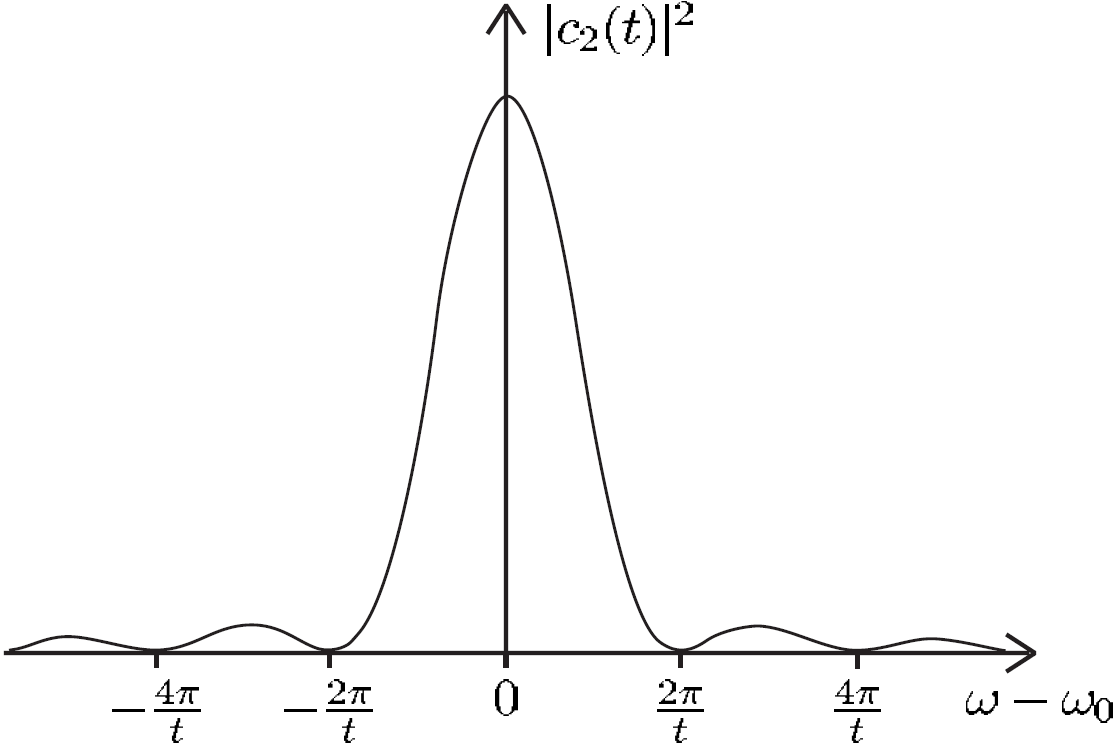
\includegraphics[width=0.75\textwidth]{Q03/images/ExcitationProbabilityFunction.PNG}
    \caption{Excitationssandsynligheden er størst idet, at det indsendte lys har en frekvens $\omega$, som stort set matcher atomets ræsonansfrekvens $\omega_0$. Functionens bredde er invers proportional med tiden, hvorfor sandsynligheden vil falde som tiden går.}
    \label{fig:Q03_ExcitationProbabilityFunction}
\end{figure}


\paragraph{Resultatets sammenhæng med spektroskopiske eksperimenter:} \ldots

\section[Atom-lysvekselvirkning i Blochvektorformalisme]{Discuss the coherent interaction between atoms and light using the Bloch vector formalism. Give an example for experiment which can be described using the Bloch vector.}

\noindent
\Large

\normalsize
\subsection{Discuss the coherent interaction between atoms and light using the Bloch vector formalism. Give an example for experiment which can be described using the Bloch vector.}


Vi kigger på et toniveausystem, hvor bølgefunktionen for dette system vil være
\begin{align} \label{eq:Q04_TotalBoelgefunktionTidsafhaengig}
    \Psi(\Vec{r},t) &= c_1\ket{1}\exp{-i\omega_1 t} + c_2\ket{2}\exp{-i\omega_2 t} \: ,
\end{align}
hvor $c_j = c_j(t)$ og $\omega_j = E_j/\hbar$ for $j = 1,\,2$.

Påvirkes dette toniveausystem nu af elektromagnetisk stråling (lys) fra et oscillerende elektrisk felt $\Vec{E} = \Vec{E}_0$ resulterer dette i perturbationen
\begin{align}
    H'(t) &= e\Vec{r} \cdot \Vec{E}_0 \cos(\omega t) \: .
\end{align}
Dette leder til et induceret dipolmoment ifølge \textsf{dipolapproksimationen}\footnote{Et atom kan approksimeres til at være en dipol. Dipolapproksimationen holder så længe, at lysets bølgelængde er større end atomet, $\lambda \gg a_0$.} Vi lader nu lyset være polariseret langs $x$-aksen, hvorved komponenten af dipolen langs denne akse vil være givet ved forventningsværdien
\begin{align} \label{eq:Q04_ElektronladningGangeInduceretDipolmoment}
    -eD_x(t) = -\bra{\Psi(t)}ex\ket{\Psi(t)} = -e\left(c_2^*c_1X_{21}\exp{i\omega_0 t} + c_1^*c_2Z_{12}\exp{-i\omega_0 t}\right) \: ,
\end{align}
hvor $\omega_0 = \omega_2 - \omega_1 = \Delta \omega$ og $X_{ij} = \bra{i}x\ket{j}$, idet der er gjort brug af bølgefunktionen fra \cref{eq:Q04_TotalBoelgefunktionTidsafhaengig}. Dipolmomentet giver en reel værdi, idet $X_{ij} = \bra{i}x\ket{j} \Rightarrow X_{21} = (X_{12})^*$, og at $X_{11} = X_{22} = 0$. For at beregne dipolmomentet $D_x(t)$ induceret af det elektriske felt, da bliver vi nødt til at kende $c_1^*c_2$ og $c_2^*c_1$, hvilke er elementer i \textsf{densitetsmatricen}
\begin{align} \label{eq:Q04_DensityMatrix}
    \ketbra{\psi}{\Psi} &=
        \begin{pmatrix}
            c_1 \\
            c_2
        \end{pmatrix}
        \begin{pmatrix}
            c_1^* & c_2^*
        \end{pmatrix}
    = \begin{pmatrix}
            \abs{c_1}^2 & c_1c_2^* \\
            c_2c_1^* & \abs{c_2}^2
        \end{pmatrix}
    = \begin{pmatrix}
            \rho_{11} & \rho_{12} \\
            \rho_{21} & \rho_{22} \\
        \end{pmatrix}
    \: .
\end{align}
Her beskriver diagonalelementerne ($|c_1|^2$ og $|c_2|^2$) populationerne i hhv. grundtilstanden og den exciterede tilstand, mens antidiagonalelementerne (eng. the off-diagonal elements) kaldes \textsf{kohærenser} (eng. coherences) og beskriver systemet ved drivfrekvensen (\cref{eq:Q04_ElektronladningGangeInduceretDipolmoment}).

Vi definerer nu to nye variable (for at fjerne den trivielle fase)
\begin{align}
    \widetilde{c}_1 &= c_1\exp{-\frac{i\delta t}{2}} \: , \\
    \widetilde{c}_2 &= c_2\exp{\frac{i\delta t}{2}} \: ,
\end{align}
hvor $\delta = \omega - \omega_0$ kaldes \textsf{detuningen}\footnote{Fordansket oversættelse af ''the detuning''.} (afvigelsen) af lysets frekvens fra atomets ræsonansfrekvens. Denne transformation ændrer ikke på populationerne, hvorfor
\begin{align}
    \widetilde{\rho}_{11} &= \rho_{11} \quad \text{og} \quad \widetilde{\rho}_22 = \rho_{22} \: ,
\end{align}
men kohærencerne ændres til
\begin{align}
    \widetilde{\rho}_{12} &= \rho_{12}\exp{-i\delta t} \quad \text{og} \quad \widetilde{\rho}_{21} = \rho_{21}\exp{i\delta t} = (\widetilde{\rho}_{12})^* \: .
\end{align}
Beskrevet ved disse nye variable bliver dipolmomentet
\begin{align}
    -eD_x(t) &= -eX_{12}\left\{u\cos(\omega t) - v\sin(\omega t)\right\} \: ,
\end{align}
hvor
\begin{align}
    u &= \widetilde{\rho}_{12} + \widetilde{\rho}_{21} \: , \\
    v &= -i\left(\widetilde{\rho}_{12} + \widetilde{\rho}_{21}\right) \: .
\end{align}
Dipolmomenter er derved nu blevet beskrevet i systemet, som roterer med vinkelfrekvens $\omega$.

Ved at differentiere de givne densitetsmatrixelemter kan man opnå de optiske Blochligninger (ikke inkluderet spontan emission):
\begin{align} \label{eq:Q04_OpticalBlochEquations}
    \frac{\text{d}}{\text{d}t}\rho_{11} &= i \frac{\Omega}{2}\left(\widetilde{\rho}_{21} - \widetilde{\rho}_{12}\right) \: , \\
    \frac{\text{d}}{\text{d}t}\rho_{22} &= i \frac{\Omega}{2}\left(\widetilde{\rho}_{12} - \widetilde{\rho}_{21}\right) \: , \\
    \frac{\text{d}}{\text{d}t}\widetilde{\rho}_{12} &= -i\delta\widetilde{\rho}_{12} + i \frac{\Omega}{2}\left(\rho_{22} - \rho_{11}\right) \: , \\
    \frac{\text{d}}{\text{d}t}\widetilde{\rho}_{21} &= i\delta\widetilde{\rho}_{21} + i \frac{\Omega}{2}\left(\rho_{11} - \rho_{22}\right) \: ,
\end{align}
hvor $\widetilde{\rho}_{12}$ og $\widetilde{\rho}_{21}$ er defineret i det roterende system, $\widetilde{\rho}_{11} = \rho_{11}$ og $\widetilde{\rho}_{22} = \rho_{22}$, $\Omega$ er Rabifrekvensen og $\delta = \omega - \omega_0$ er detuningen.

Beskrives disse optiske Blochligninger som funktion af $u$, $v$ og $w = \rho_{11} - \rho_{22}$, da fås
\begin{align}
    \Dot{u} &= \delta v \: , \label{eq:Q04_DotU} \\
    \Dot{v} &= -\delta u + \Omega w \: , \label{eq:Q04_DotV} \\
    \Dot{w} &= -\Omega v \: . \label{eq:Q04_DotW}
\end{align}
Ved at definere \textsf{Blochvektoren} som $\Vec{R} = u\Hat{e}_1 + v\Hat{e}_2 + w\Hat{e}_3$ kan \cref{eq:Q04_DotU,eq:Q04_DotV,eq:Q04_DotW} skrives som
\begin{align} \label{eq:Q04_DotBlochVector}
    \Dot{\Vec{R}} &= \Vec{R} \cross \Vec{W} = \Vec{R} \cross \left(\Omega\Hat{e}_1 + \delta\Hat{e}_3\right) \: .
\end{align}
Her er $\Omega$ Rabifrekveensen, hvilket er den frekvens, som populationen drives med, og $\delta = \omega - \omega_0$ er detuningen.

Af \cref{eq:Q04_DotBlochVector} følger nogle vigtige egenskaber:
\begin{itemize}
    \item Grundet krydsproduktet må $\Dot{\Vec{R}} \perp \Vec{R}$, hvilket giver, at $|\Vec{R}|^2 = \text{konstant}$, og det kan vises, at $|\Vec{R}|^2 = 1$. Blochvektoren beskriver altså positionen af et punkt på en sfære med radius $1$, hvilket kaldes Blochsfæren.
    \item Grundet krydsproduktet må $\Dot{\Vec{R}} \perp \Vec{W}$, hvorfor $\Dot{\Vec{R}} \cdot \Vec{W} = 0$, så $\Vec{R} \cdot \Vec{W} = RW\cos(\theta) = \text{konstant}$. Sker der excitation med en konstant Rabifrekvens og detuning vil $W$ være konstant, og siden $R$ er fast, så vil Blochvektoren bevæge sig rundt om Blochsfæren i en cirkelbevægelse med konstant vinkel $\theta$.
\end{itemize}

\begin{figure}[!h]
    \centering
    \includegraphics[width=\textwidth]{Q04/images/BlochSphere.PNG}
    \caption{}
    \label{fig:Q04_BlochSphere}
\end{figure}


\paragraph{Ekperiment beskrivet ved Blochvektorformalismen:} \ldots Atomuret

\section{Briefly outline the solution of the Schrödinger equation for hydrogen and comment on the result. What are the separation constants and why is the energy degenerate in $l$ and $m_l$?}
\sectionmark{Schrödingerligningen for hydrogen}

\noindent
\large

\normalsize
\subsection{Tekst}

\emph{Briefly outline the solution of the Schrödinger equation for hydrogen and comment on the result. What are the separation constants and why is the energy degenerate in $l$ and $m_l$?}

\section{Discuss how the dipole approximation for the atom light interaction leads to the transition dipole moment and outline how this leads to the selection rules.}
\sectionmark{Udvalgsregler fra dipolapproksimation}

\noindent
\large

\normalsize
\subsection{Tekst}

\emph{Discuss how the dipole approximation for the atom light interaction leads to the transition dipole moment and outline how this leads to the selection rules.}

\section{Outline how the selection rules for $m$, $l$, and $s$ were obtained and explain them based on the angular momentum of the photon. Under what condition are these selection rules valid?}
\sectionmark{Udvalgsregler fra fotonens impulsmoment}

\noindent
\large

\normalsize
\subsection{Outline how the selection rules for $m$, $l$, and $s$ were obtained and explain them based on the angular momentum of the photon. Under what condition are these selection rules valid?}


Udvalgsregler (eng. selection rules) benyttes til at bestemme, hvilke overgange i et atom, som er tilladte. Mere specifikt kan disse benyttes til at beskrive, hvornår matrixelementet, som beksriver overgangssandsynligheden vil være 0, altså hvornår vi ikke behøver at udregne det sfæriske integral, og hvornår det er nødvendigt.\\


\paragraph{Udvalgsregler baseret på fotonens impulsmoment:} Udvalgsreglen for $l$ kan vi også finde ud fra vekselvirkningen med en foton, idet fotonen har et impulsmoment på $1$ (i enheder af $\hbar$). Idet fotonen vekselvirker med en elektron optagere denne fotonen og dermed også dens impulsmoment, så grundet impulsmomentbevarelse må der ske end ændring med $\Delta l = \pm 1$, hvor fortegnet skyldes retningen af fotonens impulsmoment i forhold til elektronens.\\
Udvalgsreglen for $m$ ($\Delta m = 0,\, \pm 1$) kan ses som værende fotonens impulsmoment langs $z$-aksen, så vi kan enten have impulsmomentet op eller ned ($\Delta m = \pm 1$) eller i en anden retning ($\Delta m = 0$).\\
Impulsmomentbevarelse forklarer dog ikke, hvorfor $\Delta l \ne 0$, hvilket kommer af pariteten\footnote{Læs \textit{Atomic Physics} af Christopher J. Foot, afsnit 2.2.3.}


\paragraph{Udvalgsregler fra dipolapproksimationen:} Som resultat af tidsafhængig perturbationsteori har vi Fermis gyldne regel, hvilken fortæller, at overgangsraten er proportional med kvadratet af matrixelementet af perturbationen. Hamiltonoperatoren, som beskriver den tidsafhængige vekselvirkning mellem et atom og det elektriske felt er givet ved
\begin{align}
    H' &= e\Vec{r} \cdot \Vec{E}(t) \: , \quad \text{hvor} \quad \Vec{E}(t) = |\Vec{E}_0|\Re{\exp{-i\omega t}\Hat{e}_\text{rad}} \: ,
\end{align}
hvor den elektriske dipoloperator er $-e\Vec{r}$. Denne vekselvirkning med stråling stimulerer overgange fra $\ket{1}$ til $\ket{2}$ med raten
\begin{align}
    \text{Rate} \propto |e\Vec{E}_0|^2 \abs{\int \psi_2^* (\Vec{r} \cdot \Hat{e}_\text{rad} \psi_1 \, \text{d}^3\Vec{r}}^2 \equiv \abs{e\Vec{E}_0}^2 \cross \abs{\bra{2}\Vec{r}\cdot\Hat{e}_\text{rad}\ket{1}}^2 \: .
\end{align}
Denne beskrivelse antager, at amplituden af det elektriske felt er uniform over hele atomet, sådan at den kan blive taget udenfor integralet over de atomare bølgefunktioner; altså grundet \textsf{dipolapproksimationen} ($\lambda \gg a_0$) vil $\Vec{E}_0$ ikke være afhængig af $\Vec{r}$.

Dipolmatrixelementet kan skrives som et produkt af af et radiær og et vinkelafhængig integral
\begin{align}
    \bra{2}\Vec{r}\cdot\Hat{e}_\text{rad}\ket{1} &= D_{12}\mathcal{I}_\text{ang} \: ,
\end{align}
hvor det radiære integral er
\begin{align}
    D_{12} &= \int_0^\infty R_{n_2,l_2}(r) r R_{n_1,l_1}(r) r^2 \, \text{d}r \: ,
\end{align}
og det vinkelafhængige integral er
\begin{align} \label{eq:Q07_AngularIntegral}
    \mathcal{I}_\text{ang} &= \int_0^{2\pi}\int_0^\pi Y_{l_2,m_2}^*(\theta,\phi) \Hat{r} \cdot \Hat{e}_\text{rad} Y_{l_1,m_1}(\theta,\phi) \sin(\theta) \, \text{d}\theta \, \text{d}\phi \: ,
\end{align}
hvor $\Hat{r} = \Vec{r}/r$.
Det radiære integral er normalt ikke 0, selvom det kan være meget småt for overgange mellem tilstande, hvis radiære bølgefunktioner har et lille overlap, f.eks. når $n_1$ er lille og $n_2$ er stor eller vice versa. Modsat så vil $\mathcal{I}_\text{ang} = 0$ medmindre strikse kriterier er opfyldt. Disse kriterier kaldes udvalgsreglerne.\\

Udvalgsrelgerne opstår fra det vinkelafhængige integral i \cref{eq:Q07_AngularIntegral}, hvilket indeholder afhængigheden af vekselvirkningen $\Hat{r}\cdot\Hat{e}_\text{rad}$ for en given polarisation af strålingen. Matematikken kræver, at vi udregner $\mathcal{I}_\text{ang}$ for et atom med en veldefineret kvantiseringsakse (valg til at være $z$-aksen) og for stråling, som har en veldefineret polarisation og udbredelsesretning. Dette er svarende til den fysiske situation af et atom behandlet med Zeemaneffekten fra et ekstrent magnetisk felt. Behandlingen af Zeemaneffekten som en klassisk oscillator viste, at komponenter med forskellig frekvens vil have forskellig polarisation i Zeemanopsplitningen. Vi benytter os af polariseringerne $\pi$ og $\sigma$ for hhv. lineært og cirkulært polariseret lys.

For at beregne $\mathcal{I}_\text{ang}$ omskrives enhedsvektoren $\Hat{r}$ til retningen af den inducerede dipol
\begin{align}
    \Hat{r} &= \frac{1}{r}(x\Hat{e}_x + y\Hat{e}_y + z\Hat{e}_z) = (\sin(\theta)\cos(\phi)\Hat{e}_x + \sin(\theta)\sin(\phi)\Hat{e}_y + \cos(\theta)\Hat{e}_z) \: .
\end{align}
Udtrykkes funktionerne af $\theta$ og $\phi$ ved de sfærisk harmoniske funktioner fås
\begin{align} \label{eq:Q07_SpericalHarmonicsAsCosAndSine}
    \sin(\theta)\cos(\phi) &= \sqrt{\frac{2\pi}{3}}(Y_{1,-1} - Y_{1,1}) \: , \nonumber\\
    \sin(\theta)\sin(\phi) &= \sqrt{\frac{2\pi}{3}}(Y_{1,-1} + Y_{1,1}) \: , \\
    \cos(\theta) &= \sqrt{\frac{2\pi}{3}}Y_{1,0} \: ,
\end{align}
hvilket leder til
\begin{align} \label{eq:Q07_rAsY}
    \Hat{r} \propto Y_{1,-1} \frac{\Hat{e}_x + i\Hat{e}_y}{\sqrt{2}} + Y_{1,0} \Hat{e}_z + Y_{1,1} \frac{-\Hat{e}_x + i\Hat{e}_y}{\sqrt{2}} \: .
\end{align}
Den generelle polariseringsvektor kan skrives som
\begin{align}
    \Hat{e}_\text{rad} = A_{\sigma^-} \frac{\Hat{e}_x + i\Hat{e}_y}{\sqrt{2}} + A_\pi \Hat{e}_z + A_{\sigma^+} \left(-\frac{\Hat{e}_x + i\Hat{e}_y}{\sqrt{2}}\right) \: ,
\end{align}
hvor $A_\pi$ afhænger af komponenten af det elektriske felt langs $z$-aksen, og komponenten i $xy$-planet er skrevet som en superposition af to cirkulære polarisationer med amplituder $A_{sigma^\pm}$.

fra udtrykket for $\Hat{r}$ beskrevet ved $Y_{l,m}(\theta,\phi)$, \cref{eq:Q07_rAsY}, med $l=1$ finder vi, at det inducerede dipolmoment i atomet er proportionelt med
\begin{align} \label{eq:Q07_HatRPrikERadACoefficienter}
    \Hat{r} \cdot \Hat{e}_\text{rad} \propto A_{\sigma^-} Y_{1,-1} + A_\pi Y_{1,0} + A_{\sigma^+} Y_{1,1} \: .
\end{align}


\paragraph{Udvalgsregler for $m$:} Først kigger vi på \textsf{lineært polariseret lys} ($\pi$-overgange) langs $z$-aksen. For lineært polariseret lys ser vi, af \cref{eq:Q07_HatRPrikERadACoefficienter,eq:Q07_SpericalHarmonicsAsCosAndSine}, at vil vil få $\Hat{r}\cdot\Hat{e}_\text{rad} \propto \cos(\theta)$, så
\begin{align}
    \mathcal{I}_\text{ang}^\pi &= \int_0^{2\pi}\int_0^\pi Y_{l_2,m_2}^*(\theta,\phi) \cos(\theta) Y_{l_1,m_1}(\theta,\phi) \sin(\theta) \, \text{d}\theta \, \text{d}\phi \: .
\end{align}
Vi observerer, at vi kan flytte de kun $\theta$-afhængige dele uden for $\phi$-integralet, hvorved vi får
\begin{align}
    \mathcal{I}_\text{ang} &= \int_0^\pi \cos(\theta)\sin(\theta) \int_0^{2\pi} Y_{l_2,m_2}^*(\theta,\phi) Y_{l_1,m_1}(\theta,\phi) \, \text{d}\phi \, \text{d}\theta \: ,
\end{align}
hvor
\begin{align}
    \mathcal{I}_\text{ang} &\propto \int_0^{2\pi} Y_{l_2,m_2}^*(\theta,\phi) Y_{l_1,m_1}(\theta,\phi) \, \text{d}\phi \propto \delta_{m_1,m_2} \: .
\end{align}
Det kan altså ses, at $\Delta m = 0$ for $\pi$-polarisation, hvis vinkelintegralet skal være forskelligt fra 0.\\

Nu kigges på \textsf{cirkulært polariseret lys} ($\sigma^\pm$-overgange) i $xy$-planet. Her kan det ses, fra \cref{eq:Q07_HatRPrikERadACoefficienter}, at $\Hat{r}\cdot\Hat{e}_\text{rad} \propto Y_{1,\pm 1}$, så
\begin{align}
    \mathcal{I}_\text{ang}^\pi &= \int_0^{2\pi}\int_0^\pi Y_{l_2,m_2}^*(\theta,\phi) Y_{1,\pm 1} Y_{l_1,m_1}(\theta,\phi) \sin(\theta) \, \text{d}\theta \, \text{d}\phi \: .
\end{align}
Det vides, at de sfærisk harmoniske bølgefunktioner multipliceres på følgende måde
\begin{align} \label{eq:Q07_MultiplySphericalHarmonics}
    Y_{l,m}Y_{l',m'} &= A Y_{l'+l,m'+m} + B Y_{l'-l,m'+m} \: ,
\end{align}
hvor $A$ og $B$ er konstanter hvis værdi ikke er interessant for os, hvorfor
\begin{align}
    Y_{1,\pm 1}Y_{l_1,m_1} &= A Y_{l_1 + 1,m_1 \pm 1} + B Y_{l_1-1,m_1\pm 1} \: .
\end{align}
Gøres som for den lineære polarisering og trækker $\theta$-afhængige elementer udenfor integralet, så fås $\phi$-integralet som følgende
\begin{align}
    \mathcal{I}_\text{ang} &\propto \int_0^{2\pi} Y_{l_2,m_2}^*(\theta,\phi) \left\{A Y_{l_1 + 1,m_1 \pm 1} + B Y_{l_1-1,m_1\pm 1}\right\} \, \text{d}\phi \propto A\delta_{m_1\pm1,m_2} + B\delta_{m_1\pm1,m_2} \: ,
\end{align}
hvilket giver udvalgsreglen $\Delta m = \pm 1$.\\

Udvalgsreglen for $m$ er derved $\Delta m = 0,\, \pm 1$.


\paragraph{Udvalgsregler for $l$:} For $l$ findes udvalgsreglerne nu ved at betragte vinkelintegralet, men nu bekymrer vi os kun om $\theta$-delen, da vi har fundet udvalgsreglerne baseret på $\phi$-afhængigheden. For begge typer polarisation er der tale om sfærisk harmoniske funktioner med $l = 1$ ($\Hat{r}\cdot\Hat{e}_\text{rad} \propto Y_{1,m}$), hvorved vores vinkelintegral bliver
\begin{align}
    \mathcal{I}_\text{ang}^\pi &= \int_0^{2\pi}\int_0^\pi Y_{l_2,m_2}^*(\theta,\phi) Y_{1,m} Y_{l_1,m_1}(\theta,\phi) \sin(\theta) \, \text{d}\theta \, \text{d}\phi \: .
\end{align}
Der gøres igen brug af \cref{eq:Q07_MultiplySphericalHarmonics}, hvilket giver
\begin{align}
    Y_{1,m}Y_{l_1,m_1} &= A Y_{l_1 + 1,m_1+m} + B Y_{l_1-1,m_1+m} \: ,
\end{align}
hvorved vi ud fra ortogonaliteten af de sfærisk harmoniske funktioner (som vi også gjorde de andre gange) finder
\begin{align}
    \mathcal{I}_\text{ang} &\propto A \delta{l_2,l_1+1} + B \delta{l_2,l_1-1} \: ,
\end{align}
hvorved vi ser, at udvalgsreglen for $l$ skal være $\Delta l = \pm 1$.


\paragraph{Udvalgsregler for spin:} Udvalgsreglen for spin er meget enkel. Det totale spinkvantetal ændres ikke ved overgange grundet den elektriske dipolapproksimation. I matrixelementet vil man få
\begin{align}
    \bra{\Psi_\text{final}}r\ket{\Psi_\text{initial}} \: ,
\end{align}
men operatoren $r$ virker ikke på spinet, hvorfor man vil få (''final'' skrives f og ''initial'' i)
\begin{align}
    \braket{\chi_f}{\chi_i}\bra{\psi_f}r\ket{\psi_i} \propto \delta_{f,i} \: ,
\end{align}
altså matrixelementet vil give 0, medmindre $\Delta s = 0$.

\section[Stern-Gerlach eksperimentet og elektronspin]{Describe how the Stern-Gerlach experiment led to the discovery of the spin of the electron. Which properties does the spin possess?}

\noindent
\Large

\normalsize
\subsection{Describe how the Stern-Gerlach experiment led to the discovery of the spin of the electron. Which properties does the spin possess?}


\paragraph{Opstillingen:} Stern-Gerlach eksperimentet, som kan ses på \cref{fig:Q08_SternGerlachEksperimentOpstilling}, blev udført af Stern og Gerlach i 1921, og skulle vise, at ... . Eksperimentet benytter en kollimeret stråle af sølvatomer, siden disse er neutralt ladede partikler, så man skulle ikke bekymre sig om en Lorentzkraft, som kunne afbøje partiklerne, i stedet for at vise, at partiklerne blev afbøjet relativit til deres formodede kvantiseret impulsmoment, hvor sidstnævnte ønskedes værende den dominerende faktor for resultatet af eksperimentet. Disse atomer blev sendt gennem et inhomogent magnetfelt skabt af en magnet, hvilket afbøjer atomerne grundet deres magnetiske dipolmoment, som skabes af deres impulsmoment, og dette danner et mønster på den fotografiske plade for enden af strålen (udenfor magneten).

\begin{figure}[!h]
    \centering
    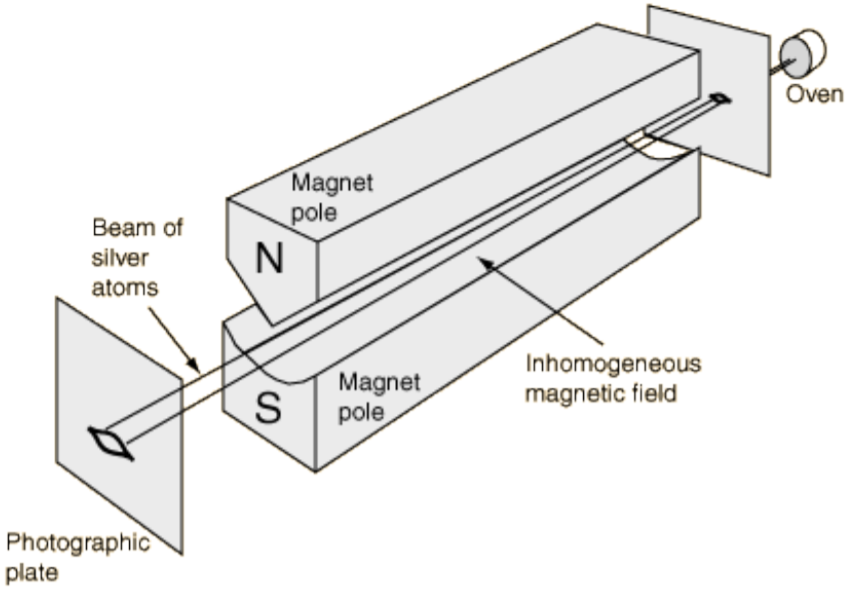
\includegraphics[width = .75\textwidth]{Q08/images/SternGerlachExperiment.PNG}
    \caption{Opstillingen af Stern-Gerlach eksperimentet.}
    \label{fig:Q08_SternGerlachEksperimentOpstilling}
\end{figure}

\paragraph{Forventning vs. resultat:} \ldots

Kigger man på forsøget med klassiske briller, så ville man forvente, at \ldots


Det blev foreslået af Uhlenbeck og Goudsmit i 1925, at elektroner havde et indre impulsmoment, også kaldet spin, hvilket viste sig at være rigtigt og kunne forklare resultatet fra Stern-Gerlach eskperimentet.

\paragraph{Egenskaber ved spin:} Spin er et impulsmoment, hvorfor det vil have de samme egenskaber som vi kender fra baneimpulsmomentet $L$:

Egenvektorerne for $\Vec{S}^2$ og $\Vec{S}_z$ vil være givet ved
\begin{align}
    \Vec{S}^2\ket{s \, m_s} &= \hbar^2 s(s+1) \ket{s \, m_s} \label{eq:Q08_EgenvektorligningForS^2} \: , \\
    \Vec{S}_z\ket{s \, m_s} &= \hbar m_s \ket{s \, m_s} \label{eq:Q08_EgenvektorligningForS_z}
\end{align}

\section[Konsekvenser af elektron- og kernespin]{The electron and the nucleus are assumed to possess an angular momentum. What consequences do these angular momenta have?}

\noindent
\Large

\normalsize
\subsection{The electron and the nucleus are assumed to possess an angular momentum. What consequences do these angular momenta have?}


\ldots

\section{Outline how the spin-orbit coupling arises. Discuss the resulting splitting of the energy states for the case of hydrogen.}

\noindent
\Large

\normalsize
\subsection{Outline how the spin-orbit coupling arises. Discuss the resulting splitting of the energy states for the case of hydrogen.}


\paragraph{Spin-banekobling:}
Schrödingerligningen er en ikke-relativistisk ligning, så hvis man skal tilføje en relativistisk effekt, f.eks. spin, så skal dette manuelt gøres ved at tilføje dettes led i Hamiltonoperatoren. I stedet for at tilføje spin-banekoblingen og de relativistiske korrektioner hvert for sig, så findes disse på en og samme tid ved at gøre brug af den relativistiske ligning for det magnetiske felt, som funktion af det elektriske felt, \cref{eq:Q10_RelativistiskElektrodynamikMagnetiskOgElektriskFelt}.

For at motive brugen af en ligning for det magnetiske felt, så kigger vi på et atom, \cref{fig:Q10_SpinOrbitCouplingAtomFremDifferentPerspectives}(venstre), hvilket er illustreret, som vi kender det: En elektron i en cirkulær bane omkring en positiv kerne.
\begin{figure}[!h]
    \centering
    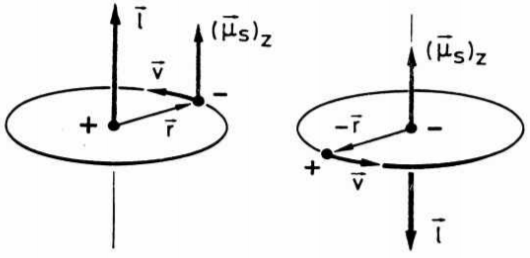
\includegraphics[width=0.7\textwidth]{Q10/images/SpinOrbiCouplingAtomFromDifferentPerspectives.PNG}
    \caption{Transformation fra kernens til elektronens perspektiv. Impulsmomentet tilhører, på begge figurer, partiklen, som er i banebevægelse, men er indtegnet ved dennes omdrejningspunkt. \textbf{Note:} Fjern fortegn fra $-\Vec{r}$ fra den højre figur, og dermed bliver $\Vec{l}$ også i retning opad i stedet.}
    \label{fig:Q10_SpinOrbitCouplingAtomFremDifferentPerspectives}
\end{figure}\\
Idet elektronen har et spin, så vil denne også have en $z$-kompenent af det magnetisk dipolmoment $\left(\Vec{\mu}_s\right)_z$. Siden elektronen er i cirkulær banebevægelse vil denne have et baneimpulsmoment $l$ (hvilket på \cref{fig:Q10_SpinOrbitCouplingAtomFremDifferentPerspectives}(venstre) er indtegnet ved elektronens omdrejningspunkt, altså atomets kerne), og dette baneimpulsmoment vil danne et magnetisk felt, som dipolmomentet så interagerer med.

Intuitivt giver det ikke mening, at elektronens dipolmoment skulle vekselvirke med elektronens dannede magnetiske felt, men dette vil give mening, når vi skifter perspektiv. Skifter vi nemlig perspektiv til at have elektronen i centrum, da vil kernen bevæge sig i cirkulær banebevægelse, hvilket vil give denne et impulsmoment, mens elektronen stadig har sit dipolmoment. Kernens impulsmoment vil nu skabe et magnetisk felt, hvilket elektronens dipolmoment vil interagere med.\\

Det giver altså mening, at vi vil kigge på den relativistiske ligning for magnetfeltet\footnote{An electron moving through an electric
field E experiences an effective magnetic field B given by this equation. This is a consequence of the way an electric field behaves under a Lorentz
transformation from a stationary to a moving frame in special relativity.}, da vi skal beskrive dipolmomentets interaktion med magnetfeltet:
\begin{align} \label{eq:Q10_RelativistiskElektrodynamikMagnetiskOgElektriskFelt}
    \Vec{B}_l &= -\frac{1}{c^2} \Vec{v} \cross \Vec{E} \: ,
\end{align}
hvor $\Vec{v}$ er elektronens hastighed.
Denne ligning kan omskrives ved at substituere $\Vec{E}$ med gradienten af potentialet og en enhedsvektor i den radielle retning (cylindriske koordinater):
\begin{align}
    \Vec{E} &= \frac{1}{e} \frac{\partial V}{\partial r} \frac{\Vec{r}}{r} \: ,
\end{align}
hvor $1/e$ kommer af, at elektrones potentielle energi $V$ er lig elektronens ladning ($-e$) gange det elektrostatiske potentiale. Derved bliver \cref{eq:Q10_RelativistiskElektrodynamikMagnetiskOgElektriskFelt}
\begin{align}
    \Vec{B}_l &= -\frac{1}{c^2} \Vec{v} \cross \left(\frac{1}{e} \frac{\partial V}{\partial r} \frac{\Vec{r}}{r}\right) = \frac{1}{c^2} \left(\frac{1}{e r} \frac{\partial V}{\partial r} \right) \Vec{r} \cross \Vec{v} = \frac{1}{m_e c^2} \left(\frac{1}{e r} \frac{\partial V}{\partial r} \right) \Vec{r} \cross m_e \Vec{v} \nonumber\\
    &= \frac{\hbar}{m_e c^2} \left(\frac{1}{e r} \frac{\partial V}{\partial r} \right) \Vec{l} \: ,
\end{align}
hvor det er blevet benyttet, at baneimpulsmomentet er $\hbar \Vec{l} = \Vec{r} \cross m_e \Vec{v}$.\\
Elektronens dipolmoment er givet ved
\begin{align} \label{eq:Q10_DipoleMomentOfAnElectron}
    \Vec{\mu}_s &= - g_s \mu_B \Vec{s} \: ,
\end{align}
hvor $g_s \simeq 2$ er Landé $g$-faktoren og $\mu_B = e\hbar/(2m_e)$ er Bohrmagnetonen.\\
Interaktionen mellem elektronens dipolmoment og det magnetiske felt giver da følgende Hamiltonoperator
\begin{align}
    H &= - \Vec{\mu}_s \cdot \Vec{B}_l = g_s \mu_B \Vec{s} \cdot \frac{\hbar}{m_e c^2} \left(\frac{1}{e r} \frac{\partial V}{\partial r} \right) \Vec{l}
\end{align}
hvilket er energien af kraftmomentet $\Vec{\mu}_s \cross \Vec{B}_l$, som den magnetiske dipol mærke i magnetfeltet $\Vec{B}_l$.

Vi har dog endnu ikke taget højde for, at vi har beregnet det magnetiske felt i et referencesystem, som ikke er statiornært, men som roterer, idet elektronen er i bevægelse omkring kernen. Dette hedder \emph{Thomas præcisionen}, og der kan tages højde for denne relativistiske effekt ved at erstatte $g_s$ med $g_s - 1$ (hvilket er $g_s - 1 \simeq 1$). Af dette fås Hamiltonoperatoren for spin-banekonlingen
\begin{align}
    H_{SO} &= (g_s - 1) \mu_B \Vec{s} \cdot \frac{\hbar}{m_e c^2} \left(\frac{1}{e r} \frac{\partial V}{\partial r} \right) \Vec{l} = (g_s - 1) \frac{e\hbar}{2m_e} \frac{\hbar}{m_e c^2} \left(\frac{1}{e r} \frac{\partial V}{\partial r} \right) \Vec{s} \cdot \Vec{l} \nonumber\\
    &= (g_s - 1) \frac{\hbar^2}{2m_e^2c^2} \left(\frac{1}{r} \frac{\partial V}{\partial r} \right) \Vec{s} \cdot \Vec{l} \: ,
\end{align}
hvor Bohrmagnetronen er indsat.\\


\paragraph{Spin-banekobling for hydrogen:}
For hydrogen er Coulombpotentialet
\begin{align}
    \frac{1}{r} \frac{\partial V}{\partial r} &= \frac{e^2}{4\pi\epsilon_0} \frac{1}{r^3} \: ,
\end{align}
så fra forventningsværdien af Hamiltonoperatoren får vi energiskiftet
\begin{align}
    E_{SO} &= \frac{\hbar^2}{2m_e^2c^2} \frac{e^2}{4\pi\epsilon_0} \braket{\frac{1}{r^3}} \braket{\Vec{s} \cdot \Vec{l} \:} \: ,
\end{align}
idet det er brugt, at $g_s - 1 \simeq 1$.

Integralet for $\braket{1/r^3}$ er givet ved
\begin{align}
    \braket{\frac{1}{r^3}} &= \dfrac{Z^3}{l\left(l+\dfrac{1}{2}\right)\left(l + 1\right) n^3a^3} \: ,
\end{align}
hvilket for hydrogen ($Z = 1$) er
\begin{align} \label{eq:Q10_<1/r^3>ForHydrogen}
    \braket{\frac{1}{r^3}} &= \dfrac{1}{l\left(l+\dfrac{1}{2}\right)\left(l + 1\right) n^3a^3} \: .
\end{align}

For at finde forventningsværdien $\braket{\Vec{s} \cdot \Vec{l} \: }$ skiftes basis til elektronens totale impulsmoment
\begin{align} \label{eq:Q10_TotalElektronimpulsmoment}
    \Vec{j} &= \Vec{l} + \Vec{s} \: ,
\end{align}
hvilket er en god basis, da Hamiltonoperatoren kommuterer med det totale elektronimpulsmoment, hvorfor $j$ er bevaret for et system uden påvirkning af eksterne kræfter. Spin-banekoblingen mellem $\Vec{l}$ og $\Vec{s}$ får disse to vektorer til at ændre deres retning samlet, således at deres sum er konstant lig $\Vec{j}$, hvorfor disse to vektoer præciserer rundt om $\Vec{j}$, som set på \cref{fig:Q10_TotalElektronimpulsmoment}.
\begin{figure}[!h]
    \centering
    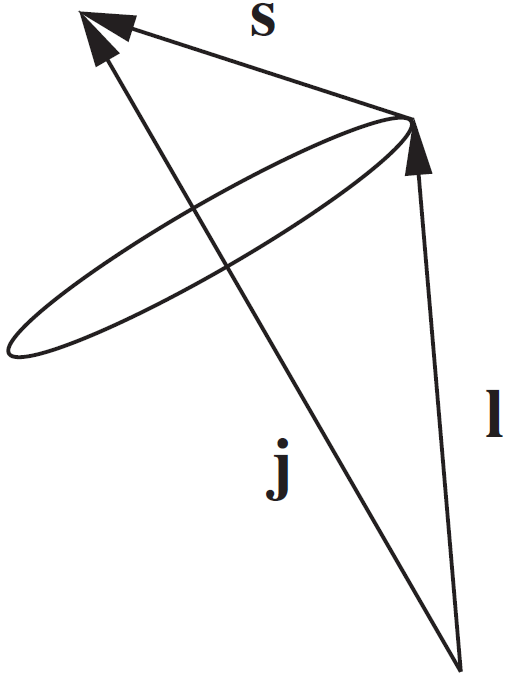
\includegraphics[width=0.23\textwidth]{Q10/images/AtomicQuantumNumberJ.PNG}
    \caption{Det totale elektronimpulsmoment $\Vec{j}$ findes som summes af baneimpulsmomentet $\Vec{l}$ og spinimpulsmomentet $\Vec{s}$, så $\Vec{j} = \Vec{l} + \Vec{s}$.}
    \label{fig:Q10_TotalElektronimpulsmoment}
\end{figure}\\
Kvadreres \cref{eq:Q10_TotalElektronimpulsmoment} fås
\begin{align}
    \Vec{j}^2 &= \Vec{l}^2 + \Vec{s}^2 + 2\Vec{s}\Vec{l} \nonumber\\
    \Rightarrow \Vec{s}\Vec{l} &= \dfrac{\Vec{j}^2 - \Vec{l}^2 - \Vec{s}^2}{2} \: ,
\end{align}
hvorfor forventningsværdien $\braket{\Vec{s} \cdot \Vec{l} \: }$ kan findes ud fra den kendte forventningsværdier $\braket{j^2}$, $\braket{l^2}$ og $\braket{s^2}$, så
\begin{align}
    \braket{\Vec{s} \cdot \Vec{l} \: } &= \frac{1}{2}\left\{j(j+1) - l(l+1) - s(s+1)\right\} \: .
\end{align}

Energiskiftet fra spin-banekoblingen bliver derved
\begin{align} \label{eq:Q10_EnergiskiftSpinOrbitForHydrogen}
    E_{SO} &= \frac{\beta}{2} \left\{j(j+1) - l(l+1) - s(s+1)\right\} \: ,
\end{align}
hvor
\begin{align}
    \beta &= \frac{\hbar^2}{2m_e^2c^2} \frac{e^2}{4\pi\epsilon_0} \dfrac{1}{l\left(l+\dfrac{1}{2}\right)\left(l + 1\right) n^3a^3} = \frac{\mu_B^2}{2c^2\pi\epsilon_0} \dfrac{1}{l\left(l+\dfrac{1}{2}\right)\left(l + 1\right) n^3a^3} \: .
\end{align}

\paragraph{Opsplitning af energitilstande i hydrogen:}

\section{Discuss the symmetry properties of the He wave functions and show which solutions are possible due to the Pauli principle.}

\noindent
\Large

\normalsize
\subsection{Tekst}

\emph{Discuss the symmetry properties of the He wave functions and show which solutions are possible due to the Pauli principle.}

\section{Describe the He spectrum (singlet and triplet states) and explain why it was initially believed that there are two kinds of helium (called para- and orthohelium).}

\noindent
\Large

\normalsize
\subsection{Tekst}

\emph{Describe the He spectrum (singlet and triplet states) and explain why it was initially believed that there are two kinds of helium (called para- and orthohelium).}

\section[Periodisk system og større atomers opbygning]{Discuss the ground states of larger atoms (up to Ne) by using Hund's first rule. Explain the general structure of the periodic table of elements (e.g. transition metals) based on the population of the electronic shells.}

\noindent
\Large

\normalsize
\subsection{Discuss the ground states of larger atoms (up to Ne) by using Hund's first rule. Explain the general structure of the periodic table of elements (e.g. transition metals) based on the population of the electronic shells.}


For at beskrive opbygningen af det periodiske system samt grundtilstanden for større atomer, så er det vigtigt at kende til Hunds første regel, og dermed også kende til Paulis udelukkelsesprincip.

\paragraph{Hunds første regel:} ''For enhver atomgrundtilstand vil det totale elektronspin have den maksimale værdi tilladt af Paulis udelukkelsesprincip.'' \footnote{For fuldstændighed, så nævnes her Hunds anden og tredje regel:
\begin{enumerate}
    \setcounter{enumi}{1}
    \item For a given multiplicity, the term with the largest value of the total orbital angular momentum quantum number $L$ has the lowest energy.
    \item For a given term, in an atom with outermost subshell half-filled or less, the level with the lowest value of the total angular momentum quantum number $J$ lies lowest in energy. If the outermost shell is more than halffilled, the level with the highest value of $J$ is lowest in energy.
\end{enumerate}
}

\paragraph{Paulis udelukkelsesprincip:} Basseret på undersøgelser af fler-elektron atomer, observerede Pauli, at de eneste atomtilstanden, som kan observeres i naturen, beskrives ved en totalbølgefunktion ($\Psi = \psi(\Vec{r})\cdot\chi(\Vec{s})$), som er antisymmetrisk under ombytning af elektronerne. En mere teoretisk tilgang til systemer med identiske partikler viser, at dette gør sig gældende ikke kun for elektroner, men for alle fermioner (partiklern med spin $n/2$, for $n\in\mathbb{N}\setminus\{0\}$, som elektroner, protoner og neutroner). Derved bliver Pauli princippet
\begin{quote}
    ''Den totale bølgefunktion for et system med mere end én identisk fermion skal altid være antisymmetrisk under ombytning af disse fermioner.''
\end{quote}
eller
\begin{quote}
    ''En atomtilstand med de tre kvantetal ($n$, $l$, $m_l$) kan maksimalt være optaget af to elektroner med modsat spin-orientering ($m_s = \pm 1/2$).''
\end{quote}
$ $\\\\

\paragraph{Opbygning af det periodiske system:} The ground state electron configuration for heavier atoms can be pieced together in much the same way. Ignoreres frastødningen indbyrdes mellem elektronerne \ldots
\noindent
Idet elektronerne er femioner er de underlagt Paulis udelukkelsesprincip, hvorfor der maksimalt kan være \emph{to} elektroner i enhver orbital -- én spin op og én spin ned, eller mere specifik skal de være i en singlet-konfiguration. Der er $n^2$ hydrogenic bølgefunktioner, som alle vil have den samme energi $E_n$, for et givet hovedkvantetal $n$, så vil $n$-skallen have plads til $2n^2$ elektroner, så for $n=1$ skallen vil der være plads til 2 elektroner, for $n=2$ skallen vil der være plads til 8 elektroner, for $n=3$ skallen vil der være plads til 18 elektroner, osv..

Kvalitativt så ville man se rækkerne i det periodiske system som svarende til at fylde en skal, men som vi kan observere af det periodiske system, så er rækkernes længde hhv. 2, 8, 8, 18, 18, osv. og ikke 2, 8, 18, 32, 50, hvilket de ville være, hvis en række blot var svarende til at fylde en hel skal. Dette skyldes vores antagelse om ignorere interaktionen mellem elektronerne. Dette problem kan vi se allerede i anden skal: Vi ved at med hydrogen og helium, så er $n=1$ skallen fyldt, så for lithium skal der en elektron i $n=2$ skallen. For $n=2$ kan impulsmomentet være $l=0$ eller $l=1$, men hvilken af disse orbitaler vil den tredje elektron lægge sig i? Uden interaktionen mellem elektronerne, da vil disse orbitaler have den samme energi, siden Bohr-energierne er afhængig af $n$ men ikke af $l$.

Interaktionenen mellem elektronerne vil favoritisere det laveste værdier af $l$, hvilket intuitivt kan forståes ved at impulsmomentet ''smider'' elektronen ud i en større bane, og jo længe ud at den kommer, jo mere blokeres kernen af de indre elektroner (effekten hedder på engelsk \emph{screening}), så man kan se det som om at de indre elektroner ser kernen med ladning $Ze$, mens den yderste elektron ser kernen med effektiv ladning $\: \sim e$, hvorfor de inderste elektroner er bedre bundet, hvorfor disse må have en lavere energi; altså må energien stige med stigende impulsmoment $l$. Så i eksemplet fra før vil lithium lægge sig s-obitalen ($l=0$), hvilket også beryllium vil, men som den næste skal bohr gøre brug af p-obitalen ($l=1$), hvilket de resterende grundstoffer op til og med neon også skal. Per Hunds første regel vil elektronerne forsøge at maksimere spinet, hvorfor de i p-obitalerne vil lægge sig i hver deres og alle være spin-op ($m_s = 1/2$), indtil der ikke er flere ledige p-obitaler i skal $n=2$, hvilket kan ses på \cref{fig:Q13_FyldningAfDeInderstseToSkaller}.

\begin{figure}[!h]
    \centering
    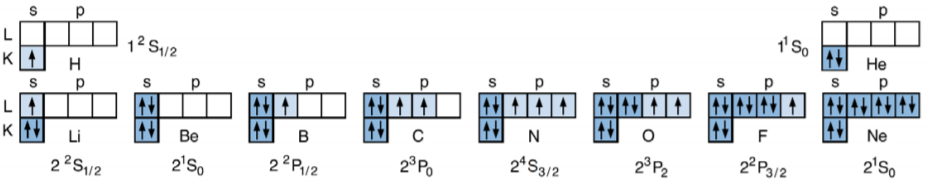
\includegraphics[width=\textwidth]{Q13/images/FirstTwoShellsElectronicSpinConfiguration.PNG}
    \caption{Princippet for opbygning af elektronkofigurationen for grundtilstanden for de første ti grundstoffer. Pilen angiver elektronens spin med $m_s = \pm 1/2$. I tilstanden, hvor der kun er én enkelt elektron kan kvantetallet for dennes spin være både $m_s = \pm 1/2$, mens den ellers vil være bestemt af den anden elektron i tilstanden, jvf. Paulis udelukkelsesprincip.}
    \label{fig:Q13_FyldningAfDeInderstseToSkaller}
\end{figure}

\paragraph{Obitalnavne:} Se \cref{tab:Q13_ImpulsmomenterOrbitalerOgDeresNavne}.
\begin{table}[!h]
    \centering
    \begin{tabular}{|c|c|c|c|c|c|c|c|c|c|c|c|}
        \hline
        $l=$ & 0 & 1 & 2 & 3 & 4 & 5 & 6 & 7 & 8 & \ldots\\
        \hline
        \textbf{Orbital} & s & p & d & f & g & h & i & k & l & \ldots \\
        \hline
        \textbf{Navn} & sharp & principal & diffuse & fundamental & & & & & &\\
        \hline
    \end{tabular}
    \caption{Impulsmomenter med tilhørenden orbitaler og deres obitalnavne.}
    \label{tab:Q13_ImpulsmomenterOrbitalerOgDeresNavne}
\end{table}

Nu har vi talt om, hvordan opbygningen af de første ti atomer er, og deres orbitaler fylder op nogenlunde logisk. I tredje skal er opfyldningen af s- og p-orbitalen stadig logisk nok, men efter argon, der fyldte sidste plads i d-orbitalen ville man formode, at man ville fylde elektroner i $3d$-orbitalen, hvilken har plads til 10 elektroner, men dette er ikke tilfældet, og $4s$-orbitaler bliver i stedet fyldt med 2 elektroner først, hvorefter $3d$-orbitalen fyldes op. Dette skyldes, at energiniveauerne her overlapper således, at $4s$-orbitalen faktisk har lavere energi end $3d$-orbitalen. Dette mønster fortsætter gennem det periodiske system, hvorfor man fylder orbitalerne som set på \cref{fig:Q13_FyldningAfSkaller}, og man kan se det i forbindelse med det periodiske system som \cref{fig:Q13_OpfyldningAfSkallerMedPeriodiskSystem}.
\noindent
Hvis det er helt rigtigt, så er der nogle småting ved opfyldningen af grundstoffet lige før (i s-orbitalen) og efter (i d-orbitalen) både lataniderne og aktaniderne, som lige mellem disse to (før og efter) springer ned og fylder med første grundstof fra lataniderne eller aktaniderne (alt efter hvilke grundstoffer, som vi taler om) i f-orbitalen. Dette kan ses af \cref{fig:Q13_FyldningAfSkallerFaktisk}.

\begin{figure}[!h]
    \centering
    \begin{subfigure}[t]{\textwidth}
        \centering
        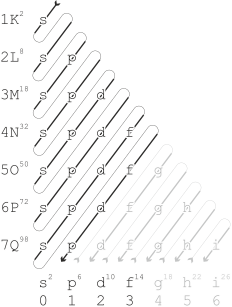
\includegraphics[width=0.5\textwidth]{Q13/images/FyldningAfSkaller3.png}
        \caption{Skallerne fyldes efter følgende møster (med små afvigelser som vist på \cref{fig:Q13_FyldningAfSkallerFaktisk}).}
        \label{fig:Q13_FyldningAfSkaller1}
    \end{subfigure}
    \vfill
    \begin{subfigure}[t]{\textwidth}
        \centering
        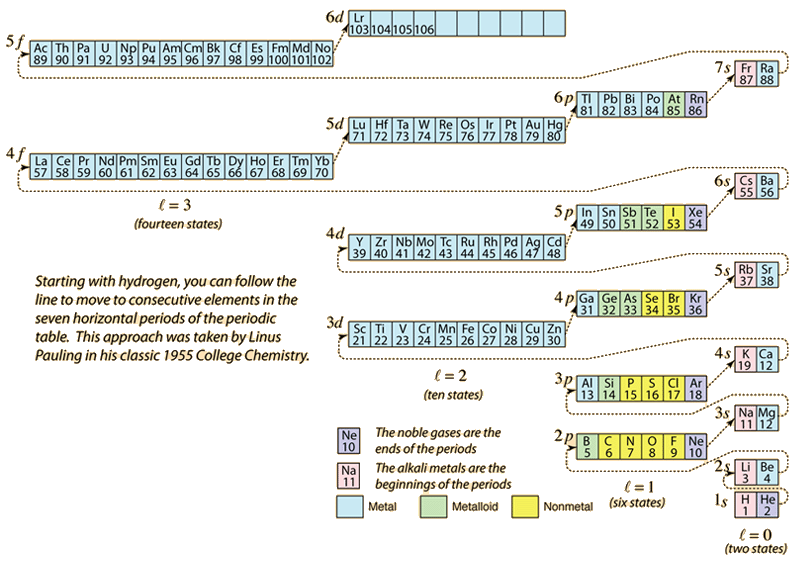
\includegraphics[width=\textwidth]{Q13/images/FyldningAfSkaller2.png}
        \caption{De forskellige orbitaler er her vist liggende i rækkefølge efter deres respektive energi (not to scale).}
        \label{fig:Q13_FyldningAfSkaller2}
    \end{subfigure}
    \caption{Opfyldning af orbitaler.}
    \label{fig:Q13_FyldningAfSkaller}
\end{figure}

\begin{figure}[!h]
    \centering
    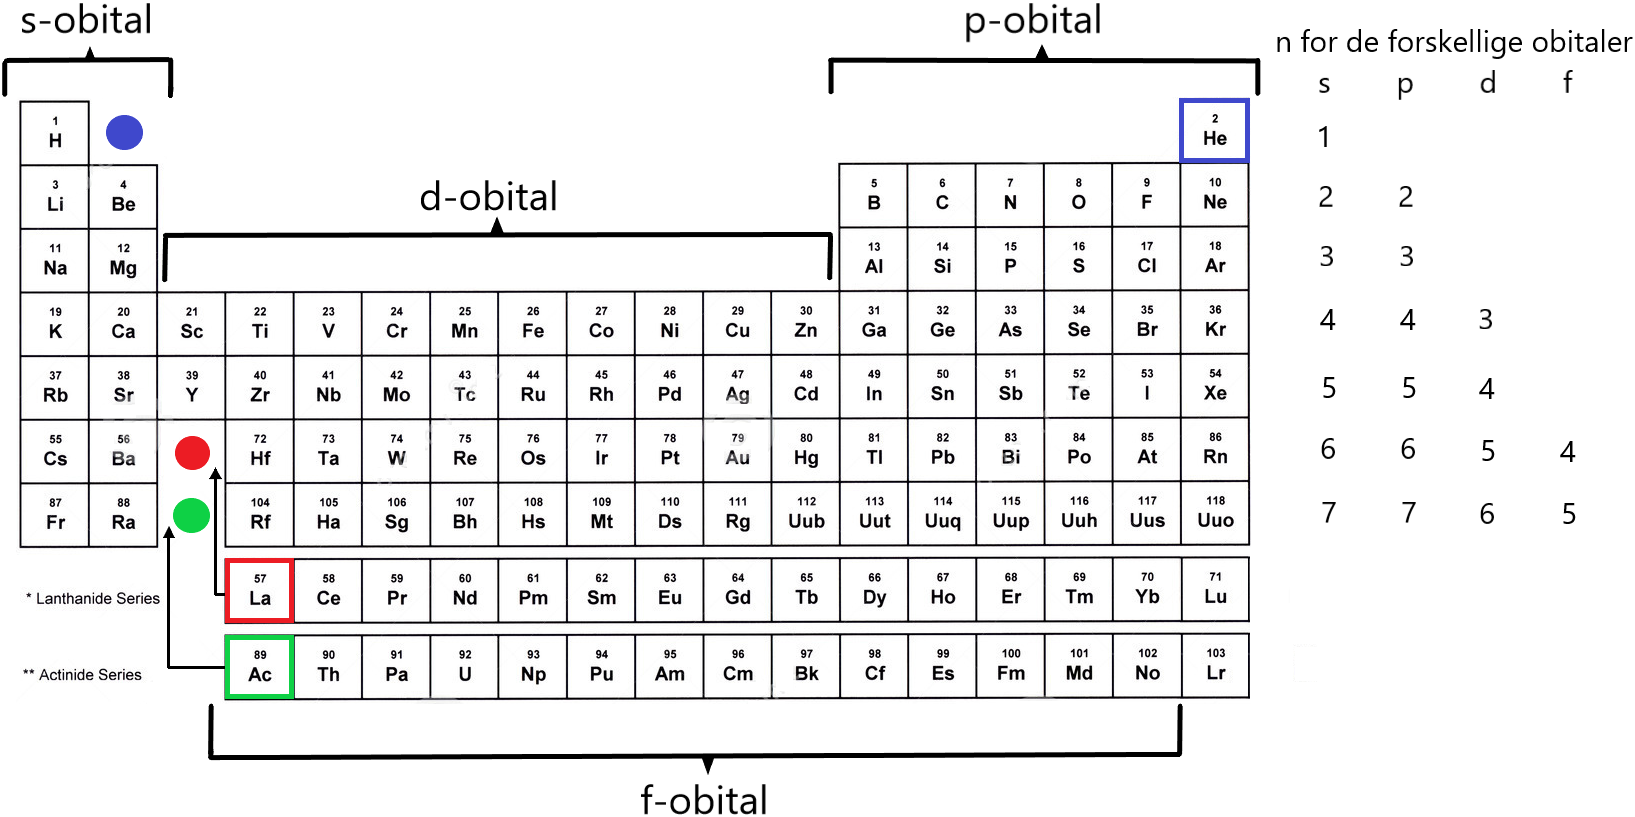
\includegraphics[width=\textwidth]{Q13/images/PeriodicTable.png}
    \caption{\cref{fig:Q13_FyldningAfSkaller} kan også visualiseres direkte i det periodiske system. Her kan det tydeligt ses, at man ikke kan se en række i det periodiske system som opfyldningen af én enkelt skal.}
    \label{fig:Q13_OpfyldningAfSkallerMedPeriodiskSystem}
\end{figure}
$ $\\\\

\paragraph{Generelt om det periodiske system:}
\begin{itemize}
    \item Det periodeske system er arrangeret efter protonnummeret $Z$, hvilket for et ikke ioniseret atom også vil være lig antallet af elektroner.
    \item Herefter er atomerne inddelt i hovedgrupper (1-8), afhængig af Hunds regel, som sørger for, at hver gruppe har lige mange valenselektroner (elektroner i yderste skal), f.eks. har alkalimetaller kun 1 valenselektron, hvorfor de ligger i hovedgruppe 1.
    \begin{itemize}
        \item Fra række 3 findes der mellem hovedgruppe 2 og 3 undergrupperne I-X.
    \end{itemize}
    \item Herefter er grundstofferne også inddelt i 7 rækker, også kaldet skaller, som for s- og p-orbitaler stemmer overens med hovedkvantetallet $n$, og som for d-orbitaler er foskudt med én, således at 3d-orbitalerne ligger i række 4, mens det for f-orbitalerne er forkudt med to, således at 4f-orbitalerne ligger i række 6.
\end{itemize}


\newpage

\begin{figure}[!h]
    \centering
    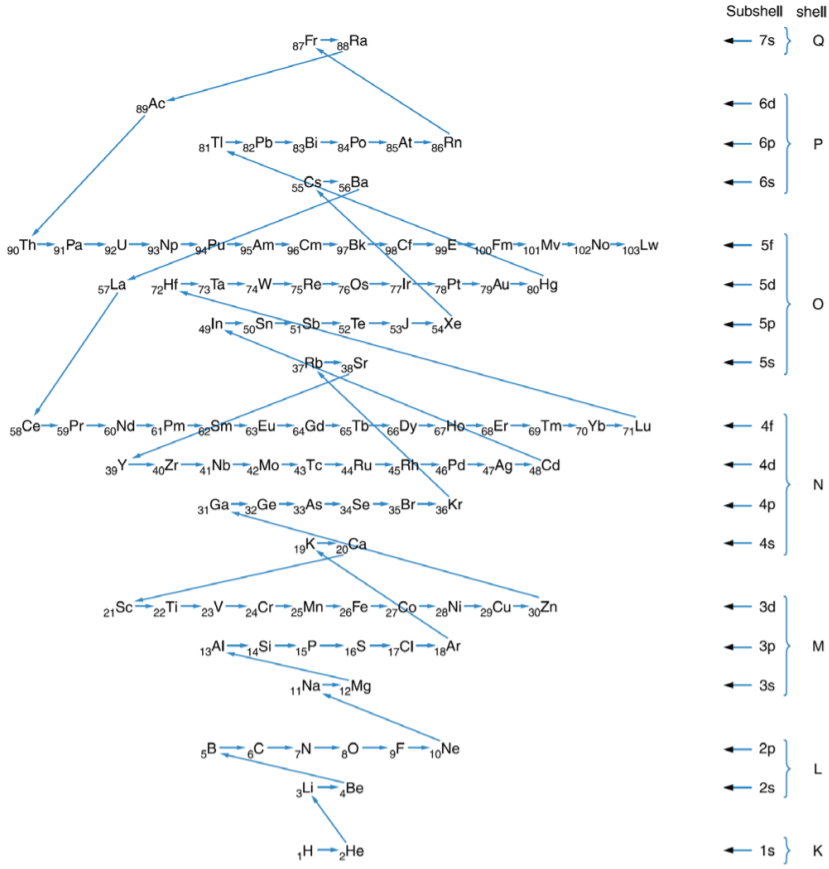
\includegraphics[width=\textwidth]{Q13/images/FyldningAfSkaller.PNG}
    \caption{Faktisk opfyldning af orbitaler, hvilket stort set, med kun få undtagelser, er det samme som vist i \cref{fig:Q13_FyldningAfSkaller}.}
    \label{fig:Q13_FyldningAfSkallerFaktisk}
\end{figure}

\section{Explain the term symbol (assuming L-S coupling) which describes the state of a multi-electron atom. Use an alkali atom to give an example.}
\sectionmark{Termsymbolet}

\noindent
\large

\normalsize
\subsection{Explain the term symbol (assuming L-S coupling) which describes the state of a multi-electron atom. Use an alkali atom to give an example.}


\paragraph{L-S kobling:} \ldots

Det totale impulsmoement bliver da $\Vec{J} = \Vec{L} + \Vec{S}$, hvor $\Vec{L} = \sum_i \Vec{l}_i$ er det totale baneimpulsmoment og $\Vec{S} = \sum_i \Vec{s}_i$ er det totale spin.

\paragraph{Termsymbol:} Termsymbolet\footnote{Dette er en fordansket betegnelse af det engelske \emph{term symbol}, men jeg er ikke bekendt med den danske betegnelse.} er en effektiv, kort og kompakt måde at skrive en stor del af den vigtigste information omkring et atom. For atomer, for hvilke L-S kolbingen gælder, kan termsymbolet skrives som
\begin{align}
    n^{2S+1}L_J \: ,
\end{align}
hvor $n$ er hovedkvantetallet, $2S+1$ er multipliciteten, altså antallet af $J$-tilstande, og
\begin{align}
    J = \abs{L - S}, \: \abs{L - S}, \: \ldots \: , \abs{L + S} - 1 \: , \abs{L + S} \: , 
\end{align}
er det totale impulsmoment. Både $n$, $S$ og $J$ skrives med deres respektive tal, mens $L$ skrives som den tilhørende orbital, se \cref{tab:Q14_ImpulsmomenterOrbitalerOgDeresNavne}.
\begin{table}[!h]
    \centering
    \begin{tabular}{|c|c|c|c|c|c|c|c|c|c|c|c|}
        \hline
        $L=$ & 0 & 1 & 2 & 3 & 4 & 5 & 6 & 7 & 8 & \ldots\\
        \hline
        \textbf{Orbital} & S & P & D & F & G & H & I & K & L & \ldots \\
        \hline
        \textbf{Navn} & Sharp & Principal & Diffuse & Fundamental & & & & & &\\
        \hline
    \end{tabular}
    \caption{Impulsmomenter med tilhørenden orbitaler og deres obitalnavne.}
    \label{tab:Q14_ImpulsmomenterOrbitalerOgDeresNavne}
\end{table}

Som eksempel kan man kigge på natrium ($Z=11$), hvilket er et alkalimetal, hvilket vil sige, at det kun har én enkelt valenselektron (elektron i yderste skal), hvilken er uparret. De to indre skaller ($n=1$ og $n=2$) er fyldt, og ved brug af Hunds regler\footnote{Hunds regler:
\begin{enumerate}
    \item For enhver atomgrundtilstand vil det totale elektronspin have den maksimale værdi tilladt ad Paulis eksklusionsprincip.
    \item For en given multiplicitet, og dermed for et bestemt spin $S$, vil den laveste energitilstand være svarende til termen med det største baneimpulsmoment $L$.
    \item For a given term, in an atom with outermost subshell half-filled or less, the level with the lowest value of the total angular momentum quantum number $J$ lies lowest in energy. If the outermost shell is more than halffilled, the level with the highest value of $J$ is lowest in energy.
\end{enumerate}
} kan vi bestemme, at den uparede elektron vil være i $3S$-orbitalen, og siden, at elektronen ligger i $S$-orbitalen, da må $L = 0$, og siden, at vi har tale om en enkelt elektron, da vil $S = 1/2$, så vi vil få $J = L + S = 0 + 1/2 = 1/2$. Derved bliver termsymbolet
\begin{align}
    n^{2S+1}L_J
\end{align}
$ $\\\\

\ldots (Der sker vist et eller andet med ''In alkali metals, the atoms only have a single, unpaired electron in the outermost shell, the rest are filled (w.
exception of some of the outermost shells, due to the quantum defect in the central-field approximation).''



$ $\\\\
BØR DER SKRIVES MERE TIL DETTE SPØRGSMÅL???

\section{How does an external magnetic field affect an atom in LS-coupling? Describe the Zeeman effect without accounting for the nucleus.}

\noindent
\Large

\normalsize
\subsection{How does an external magnetic field affect an atom in LS-coupling? Describe the Zeeman effect without accounting for the nucleus.}


\paragraph{LS-kobling:}


\paragraph{Zeemaneffekten med LS-kobling:}

\section{Outline the origin of the hyperfine structure. What are the assumptions made for the nucleus? Discuss the resulting splitting of the energy states.}
\sectionmark{Hyperfinstruktur}

\noindent
\large

\normalsize
\subsection{Outline the origin of the hyperfine structure. What are the assumptions made for the nucleus? Discuss the resulting splitting of the energy states.}


Ligesom elektronen har protonerne og neutronerne i kernen også et spin, da alle elementarpartikler har dette, og der tages nu højde for, at kernen også har et spin, kaldet \textsf{kerneimpulsmoment} $I$ (eng. nuclear angular momentum). Som andre impulsmomenter giver kerneimpulsmomentet anledning til et magnetisk dipolmoment
\begin{align} \label{eq:Q16_NuclearAngularMomentumMagneticMoment}
	\vec{\mu}_I &= g_N \frac{\mu_N}{\hbar} \vec{I} \: ,
\end{align}
hvor der, modsat elektronens dipolmoment, ikke er et negativt fortegn, da dette stammer fra elektrones ladning\footnote{Hvis masse og ladning er fordelt identisk, så er faktoren $\gamma$ ($\vec{\mu} = \gamma \vec{L}$ for et impulsmoment $\vec{L}$) givet som $\frac{q}{2m}$, hvor $q$ er partiklens ladning og $m$ dens masse.}. I \cref{eq:Q16_NuclearAngularMomentumMagneticMoment} er $\mu_N = e\hbar/(Zm_p)$ kernemagnetronen (eng. nuclear magnetron). Kernen har et meget mindre dipolmoment end elektronerne, da kernemagnetronen er meget mindre end Bohrmagnetronen\footnote{Bohrmagnetronen er givet ved $\mu_B = \frac{e\hbar}{4m_e}$.}
\begin{align}
	\mu_B &= \frac{m_p}{m_e}\mu_N = 1836 \mu_N \: .
\end{align}

Af denne grund kan $H_{HFS}$ ses som en perturbation, og denne beregnes ved
\begin{align} \label{eq:Q16_HyperFineStructureHamiltonStart}
	H_{HFS} &= -\vec{\mu}_I \cdot \vec{B}_J
	= -\left(g_N \frac{\mu_N}{\hbar} \vec{I}\right) \cdot \left(-B_J \frac{\vec{J}}{\abs{\vec{J} \: }}\right)
	= g_N \frac{\mu_N}{\hbar} B_J \frac{\vec{I} \cdot \vec{J}}{\abs{\vec{J} \: }} \: ,
\end{align}
hvor det er benyttet, at det magnetiske felt dannet af elektronen $\vec{B}_J = - B_J \vec{J}/|\vec{J}|$, hvor fortegnet kommer fra, at vi har beregnet det magnetiske felt ved kernes position, som er $-\vec{r}$ set fra elektronens synspunkt. Et magnetisk felt i $\vec{J}$-retnignen skyldes, at vi i vektormodellen vil se en hurtig præcision omkring $\vec{J}$, og derfor vil enhver anden komponent end dem langs med $\vec{J}$ tidsgennemsnitlig være $0$ (vi lader altså det magnetiske felt projiceres ind på $\vec{J}$)\footnote{Larmorpræcisionen?}. Hermed kan energiskiftet grundet hyperfinstrukturen beregnes som
\begin{align} \label{eq:Q16_HyperFineStructureEnergyChangeStart}
    E_{HFS} &= \braket{H_{HFS}} = g_N \frac{\mu_N}{\hbar} B_J \braket{\frac{\vec{I} \cdot \vec{J}}{\abs{\vec{J} \: }}} \: .
\end{align}

Vi skifter nu basis til det totale atomarimpulsmoment $\vec{F} = \vec{I} + \vec{J}$, da kerneimpulsmomentet og det totale elektronimpulsmoment er koblede. Fra dette kan vi nu finde $\braket{\vec{I} \cdot \vec{J} \:}$
\begin{align}
    \Vec{F}^2 &= \Vec{I}^2 + \Vec{J}^2 + 2\Vec{I} \cdot \Vec{J} \nonumber\\
    \Rightarrow \braket{\Vec{I} \cdot \Vec{J}} &= \frac{1}{2} \left(\braket{\Vec{F}^2} - \braket{\Vec{I}^2} - \braket{\Vec{J}^2}\right) = \frac{\hbar^2}{2} \left\{F(F+1) - I(I+1) - J(J+1)\right\} \: ,
\end{align}
og vi ved, at $\braket{|\vec{J}|} = \hbar \sqrt{J(J+1)}$, hvorfor energiskiftet i \cref{eq:Q16_HyperFineStructureEnergyChangeStart} bliver til
\begin{align} \label{eq:Q16_HyperFineStructureEnergyChange}
    E_{HFS} &= g_N \frac{\mu_N}{\hbar} B_J \frac{\hbar^2}{2\hbar} \frac{F(F+1) - I(I+1) - J(J+1)}{\sqrt{J(J+1)}} \nonumber\\
    &= \frac{A}{2}\left\{F(F+1) - I(I+1) - J(J+1)\right\} \: , \quad \text{hvor} \quad A = \frac{g_N \mu_N B_J}{\sqrt{J(J+1)}} \: .
\end{align}
Her er $A$ \textsf{hyperfinstrukturkonstanten} og det resterende kaldes \textsf{intervalfaktoren}. \textbf{Note:} I $B_J$ er Bohrmagnetronen $\mu_B$ indeholdt.


\paragraph{Opsplitning:} Hyperfinstrukturen vil dermed give en opsplitning til $F$-tilstande, hvorfor udartetheden (eng. degeneracy) i $J$ løftes.\\

Som eksempel kan vi se på 2P-tilstanden i hydrogen. Her er $n = 2$ og $l = 1$, og siden at vi taler om en enkelt elektron vil $s = 1/2$, hvorfor $j = 1/2,\: 3/2$. Hydrogenkernen består af en enkelt proton, hvilken har spin $1/2$, hvorfor $I = 1/2$. Derved bliver $F = 1,\: 2$ og $F = 0,\: 1$ hhv.. Dette kan ses af \cref{fig:Q16_HyperFineSplittingOf2PstateInHydrogen}.
\begin{figure}[!h]
    \centering
    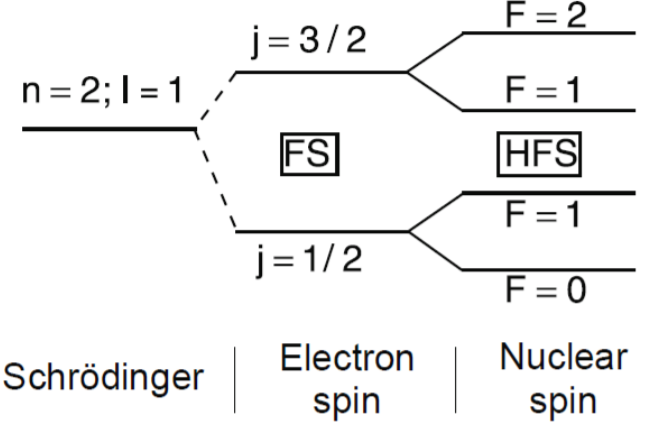
\includegraphics[width=0.60\textwidth]{Q16/images/HyperFineSplittingOf2PstateInHydrogen.PNG}
    \caption{Fin- og hyperfinstrukturopsplitning af 2P-tilstanden i hydrogen. $n = 2$, $l = 1$, så $j = \frac{1}{2}, \: \frac{3}{2}$ og $F = 0,\: 1,\: 2$. Not to scale.}
    \label{fig:Q16_HyperFineSplittingOf2PstateInHydrogen}
\end{figure}\\
Energiskiftet grundet finstrukturen vil dermed for $F = 2$ (og $j = \frac{3}{2}$) tilstanden være
\begin{align}
    E_{HFS} &= \frac{A}{2} \left\{F(F+1) - I(I+1) - J(J+1)\right\} \nonumber\\
    &= \frac{A}{2} \left\{2(2+1) - \frac{3}{2}(\frac{3}{2}+1) - \frac{1}{2}(\frac{1}{2}+1)\right\} \nonumber\\
    &= \frac{A}{2} \left\{2 \cdot 3 - \frac{3}{2} \cdot \frac{5}{2} - \frac{1}{2} \cdot \frac{3}{2}\right\} \nonumber\\
    &= \frac{A}{2} \left\{6 - \frac{15}{4} - \frac{3}{4}\right\} \nonumber\\
    &= \frac{A}{2} \left\{\frac{24}{4} - \frac{18}{4}\right\}
    = \frac{A}{2} \left\{\frac{6}{4}\right\} \nonumber\\
    &= \frac{3A}{4} \: .
\end{align}
For $F = 1$ (og $j = \frac{3}{2}$) tilstanden vil energiskiftet være
\begin{align}
    E_{HFS} &= \frac{A}{2} \left\{F(F+1) - I(I+1) - J(J+1)\right\} \nonumber\\
    &= \frac{A}{2} \left\{1(1+1) - \frac{3}{2}(\frac{3}{2}+1) - \frac{1}{2}(\frac{1}{2}+1)\right\} \nonumber\\
    &= -\frac{5A}{4} \: .
\end{align}
Dette overholder \textsf{intervalreglen}
\begin{align}
    (E_{HFS})_F - (E_{HFS})_{F-1} &= FA \: ,
\end{align}
hvilket overholdes, da
\begin{align}
    (E_{HFS})_2 - (E_{HFS})_1 &= \frac{3A}{4} - \left(-\frac{5A}{4}\right) = \frac{3A}{4} + \frac{5A}{4} = 2A \: .
\end{align}

\section{Discuss the Zeeman Effect in the presence of hyperfine structure.}

\noindent
\Large

\normalsize
\subsection{Discuss the Zeeman Effect in the presence of hyperfine structure.}


\paragraph{Zeemaneffekten:} Idet atomer opfører sig som magnetiske dipoler, da vil man observere et energiskift, hvis atomet indsættes i et eksternt magnetisk felt. Energiskiftet grundet vekselvirkningen mellem atomets dipolmoment og det eksterne magnetfelt vil løfte udartetheden (eng. the degeneracy) af tilstanden, idet man hyperfinstrukturen får en opsplitning i $M_F$.


\paragraph{Hyperfinstruktur:} Hyperfinstrukturen opstår, da man tager højde for kernens impulsmoment. Man bliver nødt til at skifte til at arbejde med det totale atomarimpulsmoment $\Vec{F} = \Vec{I} + \Vec{J}$, hvorved der skiftes basis fra $\ket{I,\: J,\: m_I,\: m_J}$ til $\ket{I,\: J,\: F,\: m_F}$. Energiskiftet grundet finstrukturen findes til at være
\begin{align}
    E_{HFS} &= \frac{A}{2}\left\{F(F+1) - I(I+1) - J(J+1)\right\} \: , \quad \text{med} \quad A = \frac{g_N \mu_N B_J}{\sqrt{J(J+1)}} \: ,
\end{align}
hvor $A$ er \textsf{finstrukturkonstanten} og det resterende kaldes \textsf{intervalfaktoren}.


\paragraph{Zeemaneffekten i hyperfinstruktur:} Som for Zeemaneffekten i finstruktur er der tre tilfælde: Hyperfinstrukturen regnes i et svagt magnetisk felt, et stærkt magnetisk felt, eller et felt med styrke midt i mellem.

\paragraph{Svagt magnetfelt:} I det svage magnetiske felt vil energiskiftet grundet Zeemaneffekten være mindre end energiskiftet grundet hyperfinstrukturen, $E_{ZE}~<~E_{HFS}$, hvorfor Zeemaneffekten kan ses som en perturbation til hyperfinstrukturen, så Hamiltonoperatoren bliver
\begin{align} \label{eq:Q17_StartudtrykForHamiltonForZeemaneffektenSvagtB}
    H_{ZE} &= - \braket{\Vec{\mu}_F} \cdot \Vec{B} \: ,
\end{align}
hvor $\braket{\Vec{\mu}_F}$ er projektionen af $\Vec{\mu}_F$ ind langs $\Vec{F}$, hvilken skal benyttes, da denne er en middelværdi af $\Vec{\mu}_F$ ($\Vec{\mu}_F$ præciserer omkring $\braket{\Vec{\mu}_F}$), og $\braket{\Vec{\mu}_F}$ er velbeskrevet i basen $\ket{I \: J \: F \: M_F}$, hvilket $\Vec{\mu}_F$ ikke er. Denne basis benyttes idet, at vi arbejder med hyperfinstruktur for svage magnetfelter, hvorfor $\Vec{I}$ og $\Vec{J}$ kobler.

Det totale magnetiske dipolmoment for et atom er givet som summen af dipolmomentet grundet elektronens spin og baneimpulsmoment og grundet kerneimpulsmomentet
\begin{align}
    \Vec{\mu}_F &= \Vec{\mu}_I + \Vec{\mu}_J = g_I \frac{\mu_N}{\hbar} \Vec{I} - g_J \frac{\mu_B}{\hbar} \Vec{J} \: ,
\end{align}
hvor $g_N$ er , $\mu_B = e\hbar/(2m_e)$ er Bohrmagnetronen, $g_I$ og $g_J$ er Landé g-faktorer for hhv. kerneimpulsmomentet og elektronimpulsmomentet (samling af baneimpulsmomentet og spinet for elektronen). Derved blive det tidsgennemsnitlige atomerdipolmoment
\begin{align}
    \braket{\Vec{\mu}_F} &= \frac{1}{\abs{\Vec{F}}^2}\left(\Vec{\mu}_F \cdot \Vec{F} \right) \Vec{F}
    = \frac{1}{\abs{\Vec{F}}^2} \left(g_I \frac{\mu_N}{\hbar} \Vec{I} \cdot \Vec{F} - g_J \frac{\mu_B}{\hbar} \Vec{J} \cdot \Vec{F}\right) \Vec{F} \: .
\end{align}

Hamiltonoperatoren fra \cref{eq:Q17_StartudtrykForHamiltonForZeemaneffektenSvagtB} bliver derved, idet $\Vec{B} = B\Hat{z}$,
\begin{align}
    H_{ZE} &= -\left\{\frac{1}{\abs{\Vec{F}}^2} \left(g_I \frac{\mu_N}{\hbar} \Vec{I} \cdot \Vec{F} - g_J \frac{\mu_B}{\hbar} \Vec{J} \cdot \Vec{F}\right) \Vec{F}\right\} \cdot \Vec{B} \nonumber\\
    &= - \frac{1}{\abs{\Vec{F}}^2} \left(g_I \frac{\mu_N}{\hbar} \Vec{I} \cdot \Vec{F} - g_J \frac{\mu_B}{\hbar} \Vec{J} \cdot \Vec{F}\right) B F_z \: ,
\end{align}
hvormed energiskiftet grundet Zeemaneffekten bliver
\begin{align} \label{eq:Q17_StartudtrykForEnergiZeemaneffetenSvagtB}
    E_{ZE,weak\,B} &= \braket{H_{ZE}} = - \frac{1}{\braket{\abs{\Vec{F}}^2}} \left(g_I \frac{\mu_N}{\hbar} \braket{\Vec{I} \cdot \Vec{F} \:} - g_J \frac{\mu_B}{\hbar} \braket{\Vec{J} \cdot \Vec{F} \:}\right) B \braket{F_z} \: .
\end{align}

Forventningsværdien af $\braket{\Vec{I} \cdot \Vec{F}}$ og $\braket{\Vec{J} \cdot \Vec{F}}$ findes ved at $\Vec{F} = \Vec{I} + \Vec{J}$, så
\begin{align}
    \Vec{J} &= \Vec{F} - \Vec{I} \Rightarrow \Vec{J}^2 = \Vec{F}^2 + \Vec{I}^2 - 2\Vec{I} \cdot \Vec{F} \nonumber\\
    \Rightarrow \braket{\Vec{I} \cdot \Vec{F}} &= \frac{1}{2} \left(\braket{\Vec{F}^2} + \braket{\Vec{I}^2} - \braket{\Vec{J}^2}\right) = \frac{\hbar^2}{2} \left\{F(F+1) + I(I+1) - J(J+1)\right\} \: , \\
    \Vec{I} &= \Vec{F} - \Vec{J} \Rightarrow \Vec{I}^2 = \Vec{F}^2 + \Vec{J}^2 - 2\Vec{J} \cdot \Vec{F} \nonumber\\
    \Rightarrow \braket{\Vec{J} \cdot \Vec{F}} &= \frac{1}{2} \left(\braket{\Vec{F}^2} + \braket{\Vec{J}^2} - \braket{\Vec{I}^2}\right) = \frac{\hbar^2}{2} \left\{F(F+1) + J(J+1) - I(I+1)\right\} \: ,
\end{align}
hvorved vi får \cref{eq:Q17_StartudtrykForEnergiZeemaneffetenSvagtB} til at blive
\begin{align} \label{eq:Q17_EnergiZeemanSvagtBfelt}
    E_{ZE,weak\,B} &= - \frac{1}{\hbar^2 F(F+1)} \frac{\hbar^2}{2}\bigg(g_I \frac{\mu_N}{\hbar} \left\{F(F+1) + I(I+1) - J(J+1)\right\} \nonumber\\
    &\qquad \qquad \qquad \qquad \quad - g_J \frac{\mu_B}{\hbar} \left\{F(F+1) + J(J+1) - I(I+1)\right\}\bigg) B \hbar M_F \nonumber\\
    &= - M_F \mu_B B \bigg(g_I \frac{\mu_N}{\mu_B} \frac{F(F+1) + I(I+1) - J(J+1)}{2F(F+1)} \nonumber\\
    &\qquad \qquad \qquad - g_J \frac{F(F+1) + J(J+1) - I(I+1)}{2F(F+1)}\bigg) \nonumber\\
    &= g_F M_F \mu_B B \: ,
\end{align}
hvor Landé g-faktoren for atomarimpulsmomentet er
\begin{align} \label{eq:Q17_gF}
    g_F \equiv g_J \frac{F(F+1) + J(J+1) - I(I+1)}{2F(F+1)} - g_I \frac{\mu_N}{\mu_B} \frac{F(F+1) + I(I+1) - J(J+1)}{2F(F+1)} \: .
\end{align}
Dette kaldes den \textsf{lineære Zeemaneffekt}.\\

Kigger vi på Rubidium-87, der har termsymbolet $5^2S_{1/2}$ og kernekvantetal $I = 3/2$, så får løfter Zeemaneffektetn udartetheden (eng. degeneracy) i $F$, som det kan ses af \cref{fig:Q17_RubidiumHyperFineZeemanSplittings}.
\begin{figure}[!h]
    \centering
    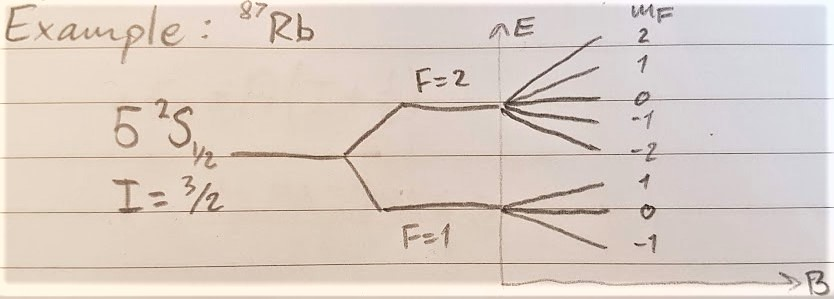
\includegraphics[width=.9\textwidth]{Q17/images/ZeemanEffectWithHyperFineStructureSplittingRubidium.jpg}
    \caption{Opsplitning af Rubidium-87 grundet Zeemaneffekten i et svagt magnetfelt.}
    \label{fig:Q17_RubidiumHyperFineZeemanSplittings}
\end{figure}


\paragraph{Stærkt magnetfelt:} I det stærke magnetfelt, $E_{ZE} > E_{HFS}$, er der tre effekter, som man kigger på
\begin{enumerate}[label=\alph*)]
    \item $\Vec{J}$ præcesserer omkring det eksterne magnetfelt.
    \item $\Vec{I}$ præcesserer omkring det eksterne magnetfelt.
    \item $\Vec{I}$ præcesserer omkring $\Vec{J}$.
\end{enumerate}

\noindent\underline{Effekt a:} Dette er Zeemaneffekten for $\Vec{J}$, hvorfor vi ved, at
\begin{align} \label{eq:Q17_EnergyFromEffectA}
    E_{\text{effect}\,a} &= g_J M_J \mu_B B \: .
\end{align}

\noindent\underline{Effekt b:} Denne effekt er meget lille og bliver derfor negligeret.

\noindent\underline{Effekt c:} Her skal hyperfinstrukturperturbationen laves igen idet, at $\Vec{I}$ og $\Vec{J}$ ikke længere indretter sig efter hinanden\footnote{Dette kaldes Pashen-Backeffekten (eng. the Pashen-Back effect): Impulsmomenterne kobler ikke længere sammen, da deres kobling til det magnetiske felt bliver stærkere end koblingen mellem de to impulsmomenter, så de nu hver især præciserer omkring det magnetiske felt i stedet for, at deres sum præciser rundt om det magnetiske felt.}.
\begin{align}
    H_{HFS,strong\,B} &= - \Vec{\mu}_I \cdot \Vec{B}_J \: ,
\end{align}
så energien bliver
\begin{align} \label{eq:Q17_EnergiStartStaerkBfelt}
    E_{HFS,strong\,B} &= \braket{H_{HFS,strong\,B}} = \braket{- \left(g_I \frac{\mu_N}{\hbar}\Vec{I}\right) \cdot \left(- B_J\frac{\Vec{J} \:}{\abs{\Vec{J}}^2}\right)} \nonumber\\
    &= g_I \frac{\mu_N}{\hbar}B_J \braket{\frac{\Vec{I} \cdot \Vec{J} \:}{\abs{\Vec{J}}^2}} \: .
\end{align}
Der er altså stadig en $\Vec{I} \cdot \Vec{J}$ interaktion, som i hyperfinstrukturen, men $\Vec{I}$ og $\Vec{J}$ orienterer sig efter det eksterne felt og ikke efter hinanden. Derved får vi ???, når $\Vec{B} = B \hat{z}$
\begin{align}
    \overline{\Vec{I} \cdot \Vec{J}} &= \left(\Vec{I}\frac{\Vec{B}}{\abs{\Vec{B}}}\right)\left(\Vec{J}\frac{\Vec{B}}{\abs{\Vec{B}}}\right) = \left(\Vec{I} \cdot \hat{z}\right)\left(\Vec{J} \cdot \hat{z}\right) = I_z J_z \\
    \Rightarrow \braket{\overline{\Vec{I} \cdot \Vec{J}}} &= \braket{I_z J_z} = M_I M_J \hbar^2 \: ,
\end{align}
så energien i \cref{eq:Q17_EnergiStartStaerkBfelt} bliver
\begin{align} \label{eq:Q17_EnergyFromEffectC}
    E_{\text{effect}\,c} &= g_I \frac{\mu_N}{\hbar}B_J \frac{\hbar^2 M_I M_J}{\hbar \sqrt{J(J+1)}} = \frac{g_I \mu_N B_J}{\sqrt{J(J+1)}} M_I M_J = A M_I M_J \: ,
\end{align}
hvor $A$ er finstrukturkonstanten.

\noindent\underline{Sammelagt:} Tilsammen bliver Zeemaneffekten for hyperfinstrukturen i stærke magnetfelter
\begin{align} \label{eq:EnergiskiftZeemanIHyperfinstrukturStarktFelt}
    E_{ZE,strong\,B} &= g_J M_J \mu_B B + A M_I M_J \: .
\end{align}
Dette kaldes den \textsf{ikke-lineære Zeemaneffekt} (eng. non-linear Zeeman effect).


\paragraph{Mellemstærkt magnetisk felt:} I mellemstræke magnetfelter er det lettere besværligt, da man skal ud i at regne udartet perturbationsteori. Der er dog et specialtilfælde for $F = I \pm I$, hvilket ses i alkalimetaller. Her kan man i stedet benytte Breit-Rabi formlen til at bestemme energiskiftet af Zeemaneffekten i hyperfinstrukturen
\begin{align}
    E_{ZE,intermediate\,B} &= - \frac{A}{4} + g_I M_F \mu_N B \pm \frac{\Delta E_0}{2} \left(1 + \frac{4M_F}{2I+1} x + x^2\right) \: ,
\end{align}
hvor
\begin{align}
    \Delta E_0 &= A\left(I + \frac{1}{2}\right) \: , \quad \text{og} \\
    x &= \frac{g_J \mu_B - g_I \mu_N}{\Delta E_0} B \: .
\end{align}



\paragraph{Zeemaneffekt i hyperfinstruktur -- Eksempel hydrogens grundtilstand:} Som eksempel kan vi kigge på finstrukturopsplitningen af hydrogens grundtilstand, hvor $I = J = 1/2$ og $g_J = g_s \simeq 2$.

I det svage magnetfelt får vi for $F = 1$, at $g_F = 1$, så denne vil nu splitte i tre energiniveauer med $M_F = -1,\: 0,\: 1$, som vil være spredt med energien $\mu_B B$ mellem dem. For $F = 0$ bliver $M_F = 0$, så der er opstår ikke en førsteordens Zeemanopsplitning. Dette kan ses af \cref{fig:Q17_AllCasesOfZeemanEffectInHyperFineStructure}.

I det stærke magnetfelt vil de to energiniveauer med $M_J = \pm 1/2$ blive opsplittet til hver to energiniveauer med $M_I = \pm 1/2$, grundet hyperfinstrukturinteraktionen. Disse energiniveauer vil være spredt med energien $A/2$ (uafhængig af magnetfeltets styrke), per \cref{eq:EnergiskiftZeemanIHyperfinstrukturStarktFelt}. Dette kan ses af \cref{fig:Q17_AllCasesOfZeemanEffectInHyperFineStructure}.

Beregning i det mellemstærke magnetfelt overlades til læseren.

\begin{figure}[!h]
    \centering
    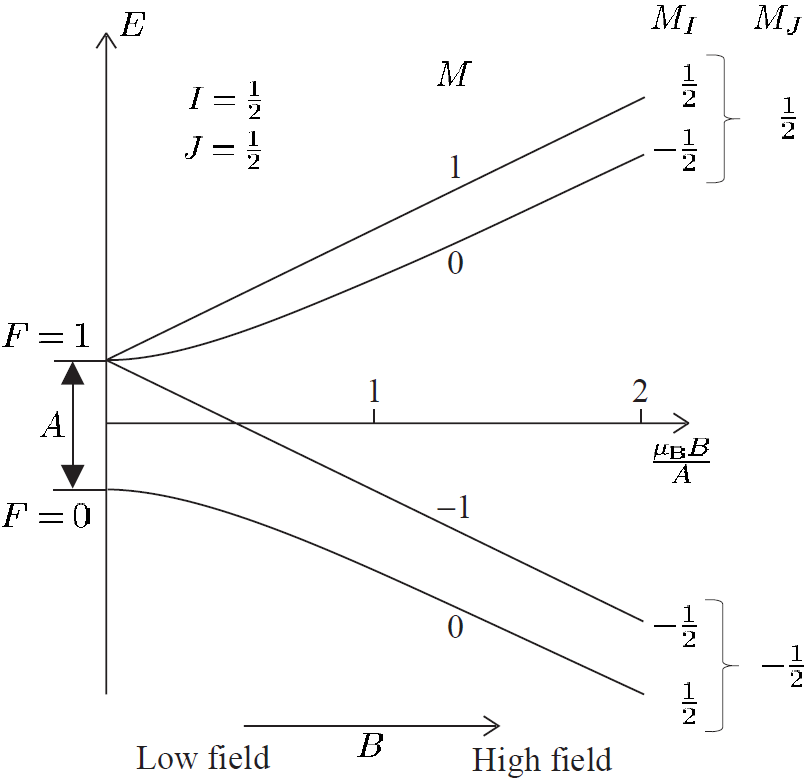
\includegraphics[width=.7\textwidth]{Q17/images/ZeemanEffectHyperFineStructurHydrogenAllCases.PNG}
    \caption{Zeemaneffektens påvirkning af hyperfinstrukturen af grundtilstanden af hydrogen ($1s\:^2 S_{1/2}$). Intervallet mellem $F=0$ og $F=1$ niveauerne  er $A$. Den horisontale akses placering midt mellem energiniveauerne skyldes, at dette hjælper på udregningerne, hvis man går i dybden med udartet perturbationsteori for det mellemstærke magnetfelt. (De to tilstande med $M_F = 0$ er i det svage magnetfelt blandet grundet perturbationen, men flytter sig fra hinanden som det magnetiske felt øges.) Værdien $x = \mu_B B/A$ er afbilledet på den horizontale akse, og svagt felt (low field) og stært felt (high field) regimerne er svarende til hhv. $x \ll 1$ og $x \gg 1$.}
    \label{fig:Q17_AllCasesOfZeemanEffectInHyperFineStructure}
\end{figure}

\section{Outline how spontaneous emission can be included in the semiclassical description of atom-light interaction and discuss the result using the optical Bloch vector.}

\noindent
\Large

\normalsize
\subsection{Outline how spontaneous emission can be included in the semiclassical description of atom-light interaction and discuss the result using the optical Bloch vector.}


I den semiklassiske beskrivelse af atom-lysinteraktion ser man lyset som værende en elektromagnetisk bølge, som beskrives klassisk, og ser atomet, som værende et toniveausystem, som er beskrevet kvantemekanisk, og man gør brug af dipolapproksimationen\footnote{Dipolapproksimationen holder så længe, at lysets bølgelængde er større end atomet, $\lambda \gg a_0$.}. Lysbølgen perturberer systemet således, at det vil begynde at oscillere mellem grundtilstanden og den exciterede tilstand, hvilket hedder \textsf{Rabioscillationer}, og disse opstår kun, når der ikke er spontan emission. Disse oscillationer kan beskrives ved Blochligningerne
\begin{align}
    \Dot{\Vec{R}} &=
        \begin{pmatrix}
            \Dot{u} \\
            \Dot{v} \\
            \Dot{w}
        \end{pmatrix}
    =
        \begin{pmatrix}
            \delta v \\
            -\delta u + \Omega w \\
            -\Omega v
        \end{pmatrix}
    = \Vec{R} \cross \left(\Omega\Hat{e}_1 + \delta\Hat{e}_3\right)
    = \Vec{R} \cross \Vec{W} \: ,
\end{align}
hvor $\delta = \omega - \omega_0$ er detuningen\footnote{Dette er en fordanskning af ''the detuning'' på engelsk.} mellem lysets frekvens og atomets resonansfrekvens, $\Omega$ er Rabifrekvensen, som driver overgange mellem de to niveauer i atomet, og $w = \rho_{11} - \rho_{22}$ er forskellen i populationen af de to niveuer.

Problemet ved denne beskrivelse er, at den ikke tager højde for spontan emission, men kun arbejder med absorption og stimuleret emission.


\paragraph{Dæmpning af en klassisk dipol:} Man kan se Rabioscillationerne som værende dreven harmonisk oscillator, hvortil man tilføjer en dæmpning, nemlig den spontane emission. Ved at betragte analogien til den klassiske dipol retfærdiggøres det, at der skal inkluderes et dæmpningsled i de optiske Blochligninger for at medtage spontan emission.

Benyttes Newtons anden lov for en harmonisk oscillator med naturlig vinkelfrekvens $\omega_0$ fås følgende bevægelsesligning
\begin{align} \label{eq:Q18_EquationOfMotionDampedHarmonicOscillator}
    \Ddot{x} + \beta \Dot{x} + \omega_0^2 x &= \frac{F(t)}{m}\cos(\omega t) \: ,
\end{align}
hvor drivkraften har amplituden $F(t)$, som ændres meget langsomt sammenlignet med oscillationen grundet drivfrekvensen, og dæmpningen er $\beta = \alpha/m$, hvor friktionskraften er givet ved $F_\text{friction} = -\alpha\Dot{x}$ og $m$ er massen.

Som løsning til \cref{eq:Q18_EquationOfMotionDampedHarmonicOscillator} ledes efter en løsning på formen
\begin{align} \label{eq:Q18_FormOfTheSolution}
    x &= \mathcal{U}(t)\cos(\omega t) - \mathcal{V}(t)\sin(\omega t) \: ,
\end{align}
hvor første led er den del af forskydningen (eng. the displacement), som er i fase med kraften, mens andet led er faseforskudt foran\footnote{A phase lead occours when $\mathcal{V}(t) > 0$, since $-\sin(\omega t) = \cos(\omega t + \pi/2)$, and $\mathcal{V}(t) < 0$ corresponds to a phase lag.} (eng. phase lead) på $\pi/2$ med hensyn til $F\cos(\omega t)$. \Cref{eq:Q18_FormOfTheSolution} forventer, at det meste af tidsafhængigheden af løsningen giver en oscillation med frekvens $\omega$. Benyttes denne løsning i \cref{eq:Q18_EquationOfMotionDampedHarmonicOscillator}, hvorefter ledene med trigonometriske funktioner forsvinder ved at ''equating the terms that depend on $\sin(\omega t)$ and $\cos(\omega t)$'', hvilket giver
\begin{align}
    \Dot{\mathcal{U}} &= (\omega - \omega_0)\mathcal{V} - \frac{\beta}{2}\mathcal{U} \: , \label{eq:Q18_DotU} \\
    \Dot{\mathcal{V}} &= -(\omega - \omega_0)\mathcal{U} - \frac{\beta}{2}\mathcal{V} - \frac{F(t)}{2m\omega} \: . \label{eq:Q18_DotV}
\end{align}
Amplituderne $\mathcal{U}$ og $\mathcal{V}$ ændrer sig med tiden som amplituden af kraften ændres, idet at vi har antaget, at kraften ændrer sig meget langsomt sammenlignet med oscillationen grundet drivfrekvensen, så må dette også gøre sig gældende for $\mathcal{U}$ og $\mathcal{V}$. Dette kaldes den \textsf{langsomtændrende konvolut-approksimation} (eng. slowly-varying envelope approximation), hvilken er blevet brugt til at udlede \cref{eq:Q18_DotU,eq:Q18_DotV}. Denne approksimation går ud på, at $\Ddot{\mathcal{U}}$ og $\Ddot{\mathcal{V}}$ er blevet negligeret\footnote{Da $\Ddot{\mathcal{U}} \sim \Ddot{\mathcal{V}} \ll 1$.}, og $\Dot{\mathcal{V}} \ll \omega \mathcal{V}$.

Den totale energi af systemet er givet som summen af den kinetiske energi ($\frac{1}{2}m\Dot{x}^2$) og den potentielle energi ($\frac{1}{2}m\omega_0^2x^2$), hvorved den totale energi bliver $E = \frac{1}{2}m\omega^2(\mathcal{U}^2 + \mathcal{V}^2)$, idet der gøres brug af approksimationen $\omega_0^2 \simeq \omega^2$, hvilken er gældende, da vi har gjort brug af en antagelse om at $\omega + \omega_0 \simeq 2\omega$ \footnote{Antagelsen er at $\omega^2 - \omega_0^2 = (\omega + \omega_0)(\omega - \omega_0) \simeq 2\omega(\omega - \omega_0)$.}, som kun gør sig gældende, når $\omega$ er tæt på resonansfrekvensen $\omega_0$. Denne energi ændres med raten $\Dot{E} = m_\omega^2(\mathcal{U}\Dot{\mathcal{U}} + \mathcal{V}\Dot{\mathcal{V}})$, og ved brug af \cref{eq:Q18_DotU,eq:Q18_DotV} bliver dette
\begin{align} \label{eq:Q18_DotE}
    \Dot{E} &= -\beta E - F \mathcal{V}\frac{\omega}{2} \: .
\end{align}
Af dette kan det ses, at hvis der ikke er en drivkraft ($F = 0$), så vil energien blot henfalde.


\paragraph{Optiske Blochligninger inkluderende spontan emission:} Et toniveausystem i et atom vil have en energi, som er proportional med populationen i den exciterede tilstand ($\rho_{22}$), $E = \rho_{22}\hbar\omega_0$, så altså $\Dot{E} \propto \Dot{\rho}_{22}$, og vi ved fra vores udregninger af de optiske Blochligninger uden spontan emission, at $\Dot{\rho}_{22} = \Omega v/2$. Sammenlignes dette med \cref{eq:Q18_DotE}, så fås
\begin{align} \label{eq:Q18_DotRho22}
    \Dot{\rho}_{22} &= -\Gamma\rho_{22} + \frac{\Omega}{2}v \: ,
\end{align}
hvor $\Gamma$ er dæmpningsledet. Af \cref{eq:Q18_DotRho22} kan det ses, at uden en Rabifrekvens ($\Omega = 0$), hvilket er drivfrekvensen, så vil populationen i den exciterede tilstand henfalde eksponentielt\footnote{Da $\Dot{x} = -kx \Rightarrow x(t) = x(0)\exp{-\Gamma t}$.}.

Sammenlignes nu $\Dot{\mathcal{U}}$ og $\Dot{\mathcal{V}}$ fra \cref{eq:Q18_DotU,eq:Q18_DotV} med $\Dot{u}$ og $\Dot{v}$ fra de optiske Blochligninger uden spontan emission, så vil de \textsf{optiske Blochligninger} indeholdende spontan emission blive
\begin{align}
    \Dot{u} &= \delta v - \frac{\Gamma}{2}u \: , \label{eq:Q18_DotLilleU} \\
    \Dot{v} &= -\delta u + \Omega w - \frac{\Gamma}{2}v \: , \label{eq:Q18_DotLilleV} \\
    \Dot{w} &= -\Omega v - \Gamma(w - 1) \: , \label{eq:Q18_DotLilleW}
\end{align}
hvilke beskriver excitationen af et toniveausystem grundet interaktion med lys, som har en frekvens tæt på atomets resonansfrekvens, for en overgang, som også kan henfalde ved spontan emission.

Vi betragter nu ligevægtsløsningen\footnote{Ligevægtsløsningen fremkommer idet man indsætter $\Dot{u} = \Dot{v} = \Dot{w} = 0$ ind i \cref{eq:Q18_DotLilleU,eq:Q18_DotLilleV,eq:Q18_DotLilleW} (eng. steady-state solution), hvilket giver tre samtidige løsninger.}, som fremkommer, når vi arbejder med tider, som er meget længere end levetiden for det øvre energiniveau, $t \ll \Gamma^{-1}$,
\begin{align}
    \begin{pmatrix}
        u \\
        v \\
        w
    \end{pmatrix}
    &= \dfrac{1}{\delta^2 + \Omega^2 / 2 + \Gamma^2 / 4}
        \begin{pmatrix}
            \Omega\delta \\
            \Omega\Gamma/2 \\
            \delta^2 + \Gamma^2 / 4
        \end{pmatrix}
        \: .
\end{align}
Disse ligninger viser, at en stærk drivfelt ($\Omega \rightarrow \infty$) vil få populationerne til at fordele sig ligeligt, idet $\rho_{11} - \rho_{22} = w \rightarrow 0$, og dette kan også ses, hvis vi betrager den exciterede population direkte
\begin{align}
    \rho_{22} &= \frac{1 - \omega}{2} = \dfrac{\Omega^2 / 4}{\delta^2 + \Omega^2 / 2 + \Gamma^2 / 4} \rightarrow \frac{1}{2} \: , \quad \text{idet} \quad \Omega \rightarrow \infty \: .
\end{align}


\paragraph{Diskussion af resultatet ved brug af Blochsfæren:} \Cref{eq:Q18_DotLilleU,eq:Q18_DotLilleV,eq:Q18_DotLilleW} kan skrives som $\Dot{\Vec{R}} = \Vec{R} \cross \Vec{W} - \Gamma \Vec{A}$, hvor $\Vec{A} = (u/2,\: v/2,\: w - 1)$. Blochvektoren $\Vec{R}$ forbliver altså den samme, mens de optiske Blochligninger blot tilføjes et dæmpningsled. Grundet dæmpningsledet, så vil Blochsfæren dog over tid blive mindre og mindre, da $\Vec{A}$'s første- og andekomponenter er parallelle med $\Vec{R}$'s, men dog af den halve længde.

\begin{figure}[!h]
    \centering
    \includegraphics[width=\textwidth]{Q18/images/BlochSphere.PNG}
    \caption{}
    \label{fig:Q18_BlochSphere}
\end{figure}

\section{Explain different physical mechanisms, which can lead to molecular binding between atoms. Which type of molecular potentials can be expected? Discuss approximations to these potentials.}
\sectionmark{Molekylære bindinger og molekylepotentialer}

\noindent
\large

\normalsize
\subsection{Explain different physical mechanisms, which can lead to molecular binding between atoms. Which type of molecular potentials can be expected? Discuss approximations to these potentials.}


Generelt er der to mekanismer, som gør at molekylære bindinger opstår mellem to neutrale atomer og lader dem sammen danne et stabilt molekyle. Vi vil se, at disse både afhænger af de specifikke atomer, men også af afstanden mellem de to kerner $R$, som set på \cref{fig:Q19_ReasonsForMolecularBinding}: Kemiske bindinger, som opstår idet, at atomernes orbitaler overlapper, og multipolvekselvirkningen, som opstår idet, at atomers opførsel som magnetiske dipoler vekselvirker med hinanden. Af kemiske bindinger vil vi kigge på de \textsf{kovalente bindinger}, og af multipolvekselvirkningerne vil vi kigge på \textsf{Van der Waals-bindinger}.\footnote{
    Ydermere findes der også følgende bindingstyper:
    \begin{itemize}
        \item \textsf{Ionbindinger} (eng. ionic bond) opstår mellem positive og negative ioner, hvis der sker en udveksling af en (eller flere) elektroner fra atom A til  således, at atom A har en lavere elektrondensitet og B en større densitet.
        \item \textsf{Hydrogenbindinger} (eng. hydrogen bond) opstår idet at der sker en ladningsforskydning mellem atomet X, som hydrogen er bundet til, og hydrogen selv, så f.eks. for vand ($\text{H}_2\text{O}$, hvor elektroner bindes tættere til oxygen end hydrogen, hvorfor der forekommer en polarisation af vandmolekylet. Hydrogen ser altså mere positiv ladning end negativ, da dens elektronsky er forskubbet mod oxygen. Et andet vandmolekyle vil derfor have lyst til at binde sig med en hydrogenbinding til det første vandmolekyle således, at det svagt negativt polariseret oxygen-atom fra det andet vandmolekyle binder sig med det svag positivt polariserede hydrogen-atom fra det første molekyle. For bindinger mellem hydrogen og et andet alkalimetal er polarisationen omvendt, så hydrogen bliver negativt polariseret, da alkalimetaller binder elektronerne svagt.
    \end{itemize}
}

\begin{figure}[!h]
    \centering
    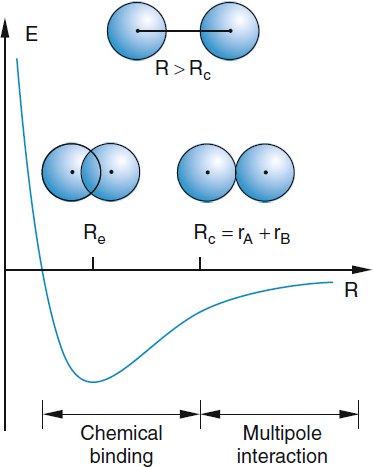
\includegraphics[width=0.45\textwidth]{Q19/images/ReasonsForBinding.PNG}
    \caption{Kemisk binding med overlab mellem atomorbitalerne er vigtig for $R < R_c$, hvor $R_c = r_A + r_B$ idet at $r_i$ er radius af atom $i$. For $R > R_c$ dominerer multipolvekselvirkningen (eng. multipole ineraction). $R_e$ er ligevægtsafstanden mellem atomerne.}
    \label{fig:Q19_ReasonsForMolecularBinding}
\end{figure}


\paragraph{Kovalente bindinger:} De kovalente bindinger opstår, når $R < R_c = \braket{r_A} + \braket{r_B}$, altså når afstanden mellem kernerne er mindre end summen af den gennemsnitlige atom radius af de to atomer. Dette er tilfældet, når de to atomers orbitaler overlapper. I dette tilfælde er der to effekter, som begge har indvirkning på bindingsenergien af molekylet (ved ligevægtsafstanden $R_e$).\\

\underline{Deling af valenselektroner:} Den første effekt, som har indvirkning, er den rummelige omstrukturering af valenselektronernes ladningsfordeling. Elektrontætheden bliver større inde mellem de to kerner, hvilket resulterer i en elektrostatisk tiltrækning mellem de positive kerner og denne negative elektrontæthed mellem kernerne. I kemisk bundne atomer deles én eller flere valenselektroner fra hvert atom i en fælles molekyleorbital. Dette er også beskrevet i \textsf{LCAO-approksimationen}, hvor den molekylære orbital er dannet af en linearkombination af atomorbitaler (eng. \textbf{L}inear \textbf{C}ombination of \textbf{A}tomic \textbf{O}rbitals).\\

\underline{Ombytningsvekselvirkning (eng. exchange interaction):} Den anden effekt er, at molekyleorbitalen har en større rummelig udstrækning end atomorbitalerne, hvilket øger den rummelige usikkerhed for elektronerne, hvorved deres gennemsnitlige impuls $\braket{|p|}$ mindskes ifølge Heisenbergs usikkerhedsprincip, og dermed også deres kinetiske energi $\braket{E_\text{kin}} = \braket{p^2}/(2m)$. Denne effekt kaldes ombytningsvekselvirkningen idet, at elektronerne i atomorbitalerne fra LCAO-approksimationen kan ombyttes, da de er identiske og dermed ikke kan skelnes i den fælles molekyleorbital.\\

Disse effekter leder sammen for stabile molekylære tilstande til et minimum i den potentielle energi $E(R)$ \footnote{Siden den potentielle energi indeholder den gennemsnitlige kinetiske energi af elektronerne.}. For afstande mindre end $R_c$ overlapper atomorbitalerne altså og danner molekyleorbitaler, hvor elektronerne deles mellem atomerne.

Betragter vi $H_2^+$, hvis bølgefunktioner kan findes ved LCAO-approksimationen, så kan man af \cref{fig:Q19_PotentialCurvesForSymmetricAndAntisymmetricWaveFunctionH2} se, at den symmetriske bølgefunktion lader et minimum eksistere i potentialet fra elektronerne, som kernerne mærker, hvilket den asymmetriske bølgefunktion ikke gør. Derved vil der være mulighed for molekylære bindinger, hvis atomerne har symmetriske bølgefunktioner og ikke asymmetriske.

\begin{figure}[!h]
    \centering
    \begin{subfigure}[t]{0.40\textwidth}
        \centering
        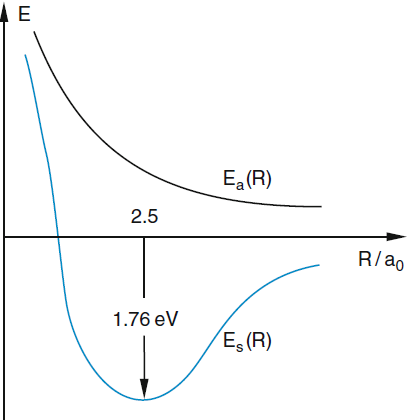
\includegraphics[width=.9\columnwidth]{Q19/images/PotentialCurvesForSymmetricAndAssymetricWaveFunctionH2.PNG}
        \caption{Potentialer.}
        \label{fig:Q19_PotentialCurvesForSymmetricAndAntisymmetricWaveFunctionH2}
    \end{subfigure}
    \hfill
    \begin{subfigure}[t]{0.45\textwidth}
        \centering
        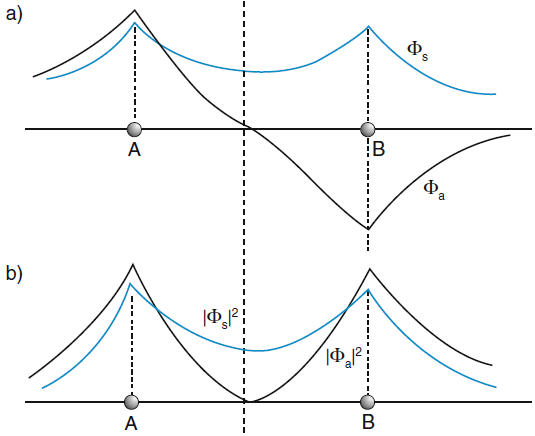
\includegraphics[width=\columnwidth]{Q19/images/SymmetriskOgAntisymmetriskBoelgefunktionForH2.PNG}
        \caption{a) $\psi^{A,S}$. b) $|\psi^{A,S}|^2$.}
        \label{fig:Q19_SymmetricAndAntisymmetricWaveFunctionsAndTheirProbability}
    \end{subfigure}
    \caption{Symmetrisk og antisymmetrisk bølgefunktion for $\text{H}_2^+$.}
    \label{fig:Q19_SymmetricAndAntisymmetricWaveFunctionsOfH2PlusIon}
\end{figure}


\paragraph{Van der Waals-bindinger:} Kovalente bindinger er de stærkeste molekylære bindinger, men grundet de er kun dominerende så længe, at der er overlap mellem atomernes orbitaler. For afstande større end $R_c$ vil der dog stadig eksistere molekylære bindinger, men disse er dog meget svagere. Dette skyldes multipolekspansionen af atomerne, og at atomerne derved har danner elektriske felter, som kan vekselvirke med hinanden. Det skal dog noteres, at potentialerne vil være afhængige af den rummelige orientering af atomerne, og om de er eller ikke er ioniserede. Nogle af disse rummelige orienteringe kan ses på \cref{fig:Q19_RummeligeOrienteringer}. Der vil være den største tiltrækning, hvis de to dipoler er parallelle, mens den største frastødning opstår, hvis de to dipoler er antiparallelle.

\begin{figure}[!h]
    \centering
    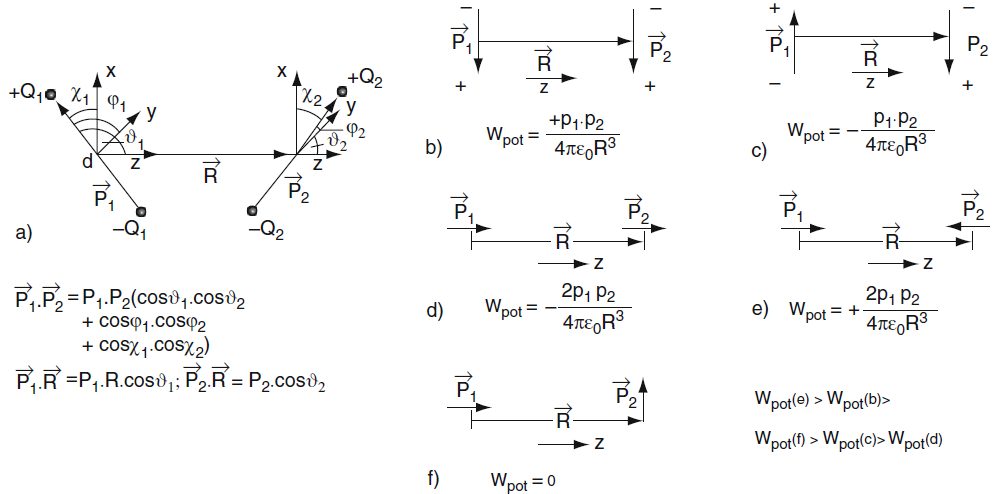
\includegraphics[width=\textwidth]{Q19/images/EnergiAfDipolerVedSpecifikkeKonfigurationer.PNG}
    \caption{Potentiel energi af to elektriske dipoler med specifikke relative orienteringer.}
    \label{fig:Q19_RummeligeOrienteringer}
\end{figure}

Placeres et neutralt atom uden et permanent dipolmoment i et elektrisk felt, så vil de modsatrettede kræfter, som påvirker de negative elektroner og den positive kerne, flytte elektronladningsfordelingen i den modsatte retning af kernen, se \cref{fig:Q19_ChargeDistributionShift}. Midtpunkterne for den positive og negative ladningsfordeling vil ikke længere være centrerede oveni hinanden, som i et neutralt atom uden et permanent dipolmoment, og dipolmomentet
\begin{align}
    \Vec{p}_A^{ind} &= \alpha_A \Vec{E}
\end{align}
induceres af det elektriske felt, og vil være parallelt med dette felt, se \cref{fig:Q19_InducedDipoleMoment}. Her er $\alpha_A$ den elektriske polarisabilitet af atom A, hvilken beskriver genoprettelseskræfterne (eng. the restoring forces) i atomet, som modvirker forskydningen og deformeringen af elektronladningsfordelingen.

\begin{figure}[!h]
    \centering
    \begin{subfigure}[t]{0.45\textwidth}
        \centering
        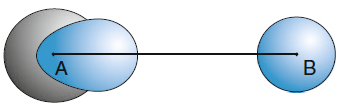
\includegraphics[width=\columnwidth]{Q19/images/ChargeDistributionShift.PNG}
        \caption{Deformation og skift af eletronladningsfordelingen fra atom A grundet vekselvirkning med atom B.}
        \label{fig:Q19_ChargeDistributionShift}
    \end{subfigure}
    \hfill
    \begin{subfigure}[t]{0.45\textwidth}
        \centering
        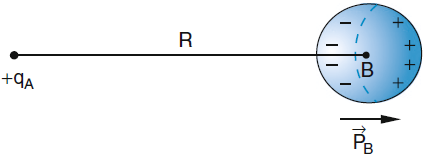
\includegraphics[width=\columnwidth]{Q19/images/InducedDipoleMoment.PNG}
        \caption{Ladningen $q_A$ inducerer et dipolmoment $\Vec{p}_B$.}
        \label{fig:Q19_InducedDipoleMoment}
    \end{subfigure}
    \caption{Inducerede dipolmomenter for to neutrale atomer.}
    \label{fig:Q_19}
\end{figure}

Hvis atomet originalt var sfærisk symmetrisk, så ville tidsgennemsnittet af dette være 0, men grundet det instantane dipolmoment, så vil et neutralt atom B i nærheden af A også have et instantant induceret dipolmoment $\Vec{p}_B^{ind} = \alpha_B \Vec{E}$, som så vil inducere et dipolmoment i atom A, og fortsat sådan. Dermed vil tidsgennemsnittet af dipolmomentet ikke længere være 0. Denne vekselvirkning mellem de to atomers momentane dipolmomenter afhænger stadig af deres rummelige orientering i forhold til hinanden, og denne effekt kaldes Van der Waals-vekselvirkning.

Den potentielle energi fra dipolvekselvirkningerne findes som
\begin{align}
    E_\text{pot}(R) &= -\Vec{p}_A^{ind} \cdot \Vec{E}_B = -\Vec{p}_B^{ind} \cdot \Vec{E}_A \: ,
\end{align}
hvor $\Vec{p}_A^{ind} = \alpha_A \Vec{E}_B$ og $\Vec{p}_B^{ind} = \alpha_B \Vec{E}_A$, hvormed den potentielle energi bliver $E_\text{pot}(R) \propto - \Vec{p}_A^{ind} \cdot \Vec{p}_B^{ind} = -\alpha_A \alpha_B \cdot |\Vec{E}|^2$, hvilket kan skrives som
\begin{align}
    E_\text{pot}(R) &= -C_1 \frac{\alpha_A \alpha_B}{R^6} = - \frac{C_6}{R^6} \: ,
\end{align}
hvor $C_1 = 1/(4\pi\epsilon_0)^2$ og $C_6 = \alpha_A \alpha_B /(4\pi\epsilon_0)^2$ er \textsf{Van der Waals-konstanten}. Dette er \textsf{Van der Waals-vekselvirkningspotentiale} (eng. Van der Waals interaction potential) mellem to neutrale atomer med polarisabiliteter $\alpha_A$ og $\alpha_B$.

\textbf{Note:} Vekselvirkningen er tiltrækkened grundet det negative fortegn, og den aftager med $1/R^6$ med stigende afstand $R$. Af denne grund er det en kortrækkende vekselvirkning sammenlignet med Coulombvekselvirkningen, som er proportionel med $1/R$, men stadig har den en længe rækkevidde end den kovalente binding, som aftager eksponentielt med stigende afstand.\\


\paragraph{Molekylepotentialer:} Mens Van der Waals-potentialet er en tilnærmelsesvis fin approksimation, så er der visse tilfælde, som den ikke tager højde for, da den negligerer højereordens multipolled, som quadropoler, oktopoler, osv.. Derudover giver den visse problemer, da der kun er et tiltrækkende led og ikke et frastødende.\\

En bedre beskrivelse vil være at gøre brug af \textsf{Lenard-Jonespotentialet}, \cref{fig:Q19_LenardJonesPotential}, som er beskrevet ved
\begin{align}
    E_\text{pot}^\text{LJ}(R) &= \frac{a}{R^12} - \frac{b}{R^6} \: ,
\end{align}
hvor $a$ og $b$ er to parametre, som afhænger af de to atomer A og B, og disse vælges til at passe bedst muligt med den eksperimentelt fundne potentalkurve, idet Lenard-Jonespotentialet er et empirisk fundet potentiale.

\begin{figure}[!h]
    \centering
    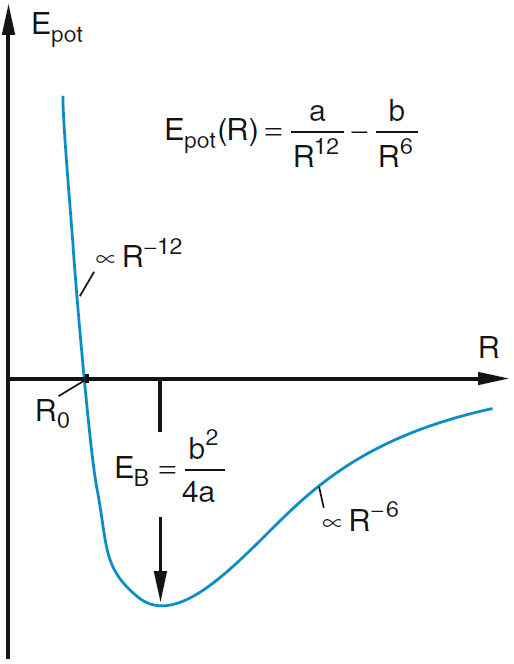
\includegraphics[width=.45\textwidth]{Q19/images/LenardJonesPotential.PNG}
    \caption{Lenard-Jonespotentialet}
    \label{fig:Q19_LenardJonesPotential}
\end{figure}\newpage
$ $\\\\

Et andet empirisk potential er \textsf{Morsepotentialet}, som har formen
\begin{align}
    E_\text{pot}(R) &= E_B \left[1 - \exp{-a(R-R_e)}\right] \: ,
\end{align}
hvilket med større præcision repræsenterer den tiltrækkende del af potentialet ift. de eksperimentelle værdier sammenlignet med det parabelpotentialet, se \cref{fig:Q19_MorsePotential}. Morsepotentialet konvergerer rigtigt nok mod adskillesesenergien (eng. the dissociation energy) for $R \rightarrow \infty$, mens parablen går mod uendelig med stigende afstand. Dog afviger Morsepotentialet mere fra det eksperimentelle potentiale for $R < R_e$ end parablen. Se \cref{fig:Q19_MorsePotential}.\\

Morsepotentialet har den store fordel, at Schrödingerligningen for to vibrerende atomer i dette potential kan blive løst præcist.

\begin{figure}[!h]
    \centering
    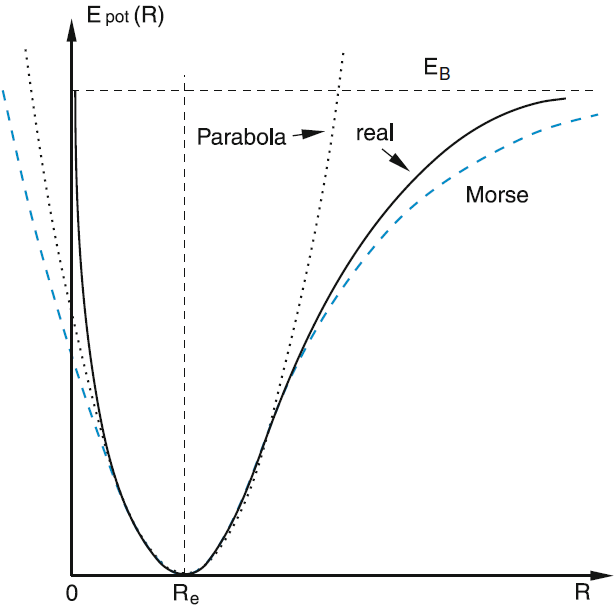
\includegraphics[width=.65\textwidth]{Q19/images/MorsePotentialComparisonWithOtherPotentials.PNG}
    \caption{Sammenligning af parabelpotentialet og Morsepotentialet med det reelle (eksperimentelle) potential.}
    \label{fig:Q19_MorsePotential}
\end{figure}

\section{Explain the origin of the molecular potential within the Born-Oppenheimer approximation and discuss the vibrational and rotational structure of diatomic molecules.}
\sectionmark{Molekylepotential i Born-Oppenheimerapproks.}

\noindent
\large

\normalsize
\subsection{Explain the origin of the molecular potential within the Born-Oppenheim approximation and discuss the vibrational and rotational structure of diatomic molecules.}


Et molekyle er ikke blot stift (eng. rigid), men det kan rotere og vibrere, hvilket vi vil tage højde for nedenfor, hvilket betyder, at vi skal tage højde for atomkernens bevægelse, når vi regner Schrödingerligningen $\Hat{H}\psi = E \psi$, hvorfor vores Hamiltonoperator nu bliver
\begin{align}
    \Hat{H} &= \Hat{H}_0 + \Hat{H}' \: , \quad \text{hvor} \quad \Hat{H}_0 = \Hat{T}_e + V \: , \quad \Hat{H}' = \Hat{T}_k \: .
\end{align}
Her er $\Hat{T}_e$ elektronernes kinetiske energi, $V$ er potentialet og $\Hat{T}_k$ er kernens kinetiske energi. Her har vi benyttet, at atomets kerne har langt større masse end elektronerne, men den bevæger sig også utrolig langsomt, og af denne grund kan det antages som en god approksimation, at elektronerne vil indrette sig instantant til kernens ændringer, hvilket giver ovenstående Hamiltonoperator. Den kinetiske energi af kernen $T_k$ er så lille, at vi ser den som værende en perturbation til den kendte Hamiltonoperator for elektronernes bevægelse $\Hat{H}_0$.
Vi kender altså løsningen til Schrödingerligningen for $\Hat{H}_0$
\begin{align}
    \hat{H}_0\phi^{el}(\Vec{r}, \Vec{R}) &= E^{(0)}(\Vec{R})\phi^{el}(\Vec{r}, \Vec{R}) \: ,
\end{align}
hvor $\phi^{el}(\Vec{r},\Vec{R})$ giver en komplet og ortogonal basis.

Vi benytter os af \textsf{Born-Oppenheimerapproksimationen}\footnote{Introduceret i 1927 af Max Born og Robert Oppenheimer.}, som negligere vekselvirkningen mellem kernens og elektronernes bevægelse, igen da elektronerne instantant indretter sig kernens bevægelser. Den totale løsning kan derfor skrives som et produkt af kernens og elektronernes bølgefunktioner
\begin{align}
    \psi(\Vec{r}, \Vec{R}) &= \sum_m \chi_m(\Vec{R}) \phi_m^{el}(\Vec{r}, \Vec{R}) \: .
\end{align}

Indsættes denne bølgefunktion i Schrödingerligningen med den fuldstændige Hamiltoperator, og multipliceres fra venstre med den $n$'te elektrons bølgefunkion, så fås
\begin{align}
    \int \left[\phi_n^{el} (\Hat{H} - E) \sum_m \chi_m\phi_m^{el}\right] \, \text{d}\Vec{r} &= 0 \: .
\end{align}
Siden vi har $\Hat{H} = \Hat{H}_0 + \Hat{H}'$, så vil integralet kunne opdeles, og den kendte løsning til Schrödingerligningen med $\Hat{H}_0$ indsættes
\begin{align}
    (E_n^{(0)} - E)\chi_n 0 + \int \phi_n^{el} \Hat{H}'\sum_m \chi_m\phi_m^{el} \, \text{d}\Vec{r} &= 0 \: ,
\end{align}
hvor det ovenstående integral kan beregnes til
\begin{align}
    &\int \phi_n^{el}\sum_m \left(\Hat{H}'\chi_m\right)\phi_m^{el} \, \text{d}\Vec{r} + \int \phi_n^{el}\sum_m \chi_m\left(\Hat{H}'\phi_m^{el}\right) \, \text{d}\Vec{r} \nonumber\\
    &\qquad \qquad \qquad \qquad \qquad \quad - \hbar \int \phi_n^{el} \sum_k \frac{1}{M_k} \sum_m \frac{\partial}{\partial R_k} \phi_m^{el} \frac{\partial}{\partial R_k} \chi_m \, \text{d}\Vec{r} \nonumber\\
    =& \int \phi_n^{el}\sum_m \left(\Hat{H}'\chi_m\right)\phi_m^{el} \, \text{d}\Vec{r} + c_{nm} \: ,
\end{align}
hvor $M_k$ er kernens masse.

Vi kan altså skrive løsningen til de to dele af den totale Hamiltonoperator som to adskilte Schrödingerligninger
\begin{align}
    \Hat{H}_0 \phi^{el}(\Vec{r}, \Vec{R}) &= E_{(0)}(\Vec{R})\phi^{el}(\Vec{r}, \Vec{R}) \: , \\
    \Vec{T}_k \chi_n(\Vec{R}) + \sigma_m c_{nm} \chi_m(\Vec{R}) &= (E - E_n^{(0)})(\Vec{R}) \chi_m(\Vec{R}) \: ,
\end{align}
og benytter vi os af Born-Oppenheimerapproksimationen ($\Rightarrow c_{nm} = 0 \: \forall n,m$) fås de følgende afkoblede ligninger
\begin{align}
    \Hat{H}_0 \phi^{el}(\Vec{r}, \Vec{R}) &= E^{(0)}(\Vec{R})\phi^{el}(\Vec{r}, \Vec{R}) \: , \\
    \Vec{T}_k \chi_n(\Vec{R}) + \sigma_m c_{nm} \chi_m(\Vec{R}) &= \{E - E_n^{(0)}(\Vec{R})\} \chi_m(\Vec{R}) \: ,
\end{align}
hvilke kan løses hver for sig, da koblingsledet er blevet negligeret.
Den første ligning beskriver en elektronbølgefunktionen for et stift (eng. rigid) molekyle, hvor elektronerne er i tilstanden $n,\, L,\, \Lambda$ og energien (uden den kinetiske energi af kernen) er $E^{(0)}$. Den anden ligning indeholder den kernens kinetiske energi $T_k$ og beskriver kernens bevægelse i potentialet $E_n^{(0)} = \braket{E_\text{kin}^{el}} + E_\text{pot}(\Vec{r}_i, \Vec{R}_k)$, hvilket, når man skifter til massemidtpunktssystemet med den reducerede masse $M = M_A M_B / (M_A + M_B)$, hvor A og B er de to atomer, giver et sfærisk symmetrisk potentiale
\begin{align} \label{eq:Q20_EquationWithSphericalSymmetricPotential}
    \left[\frac{-\hbar^2}{2M}\Vec{\nabla}^2 + E_\text{pot}^(n)(R)\right] \chi_{n,m}(\Vec{R}) &= E_{n,m}\chi_{n,m}(\Vec{R}) \: ,
\end{align}
hvor indekset $m$ giver den $m$'te kvantetilstand af kernens bevægelse (vibrations-rotationstilstanden). Det vigtige er her at notere, at der er tale om sfærisk symmetri, hvorfor potentialet kun afhænger af $R$, selvom bølgefunktionerne stadig afhænger af alle de sfæriske korrdinater.

Vi kan dog nu behandle potentialet på samme måde, som vi gjorde med hydrogenatomet, og benytter vi os af separation af variabler fås
\begin{align}
    \chi(R,\theta,\phi) &= S(R)Y(\theta,\phi) \: .
\end{align}
The radiære funktion $S(R)$ afhænger af den radiære del af potentialet og beskriver molekylets vibrationelle struktur, mens den sfæriske harmoniske funktion er løsningen til alle sfærisk symmetriske potentialer uanset deres radielle struktur, og den beskriver molekylets rotation.
Indsættes denne bølgefunktion i \cref{eq:Q20_EquationWithSphericalSymmetricPotential} findes den radiære bølgefunktion og den sfæriske harmoniske bølgefunktion
\begin{align}
    \frac{1}{\text{d}R^2}\frac{\text{d}}{R}\left(R^2 \frac{\text{d}S}{\text{d}R}\right) + \frac{2M}{\hbar^2}\left[E - E_\text{pot}(R) - \frac{J(J+1)\hbar^2}{2MR^2}\right]S &= 0 \: , \\
    \frac{1}{\sin(\theta)} \frac{\partial}{\partial \theta} \left(\sin(\theta) \frac{\partial Y}{\partial \theta}\right) + \frac{1}{\sin^2(\theta)} \frac{\partial^2 Y}{\partial \phi^2}  + J(J+1)Y &= 0 \: ,
\end{align}
hvor $J(J+1)$ er separationskonstanten.


\paragraph{Rotation:}


\paragraph{Vibration:}

\begin{figure}[!h]
    \centering
    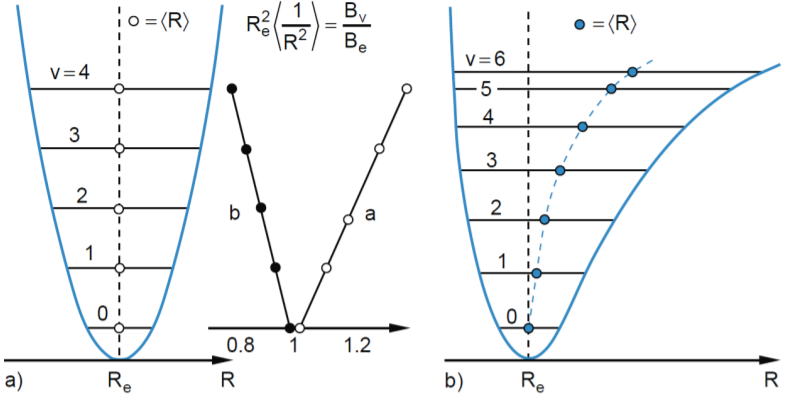
\includegraphics[width=.8\textwidth]{Q20/images/AfstandMellemEnerginiveauerneIToForskelligePotentialleApproksimationer.PNG}
    \caption{harmonisk oscillator-poteintiale sammenlignet med Morsepotentialet. Det kan ses, at afstanden mellem de vibrationelle tilstande er ens for den harmoniske oscillator, men bliver tættere og tættere end i Morsepotentialet.}
    \label{fig:Q20_AfstandMellemEnerginiveauer}
\end{figure}


\paragraph{Sammenhæng af vibration og rotation:} I virkeligheden er verden dog ikke så sort/hvid, at molekyler enten roterer eller vibrerer; de gør selvfølgelig begge dele, og deres bevægelse vil komme til at blive beskrevet som på \cref{fig:Q20_VibratingRotor}. Siden den totale energi af molekylet $E = E_\text{rot} 0 E_\text{vib} + E_\text{pot}$ skal være konstant ($\Dot{E} = 0$) må der findes en periodisk relation for ombytningen af vibrationel energi, rotationel energi og potentiel energi. Dog er det meget besværligere at løse for et sådan system, og dette kan kun gøre ved brud af mange approksimationer og udviklinger (eng. expansions).

\begin{figure}[!h]
    \centering
    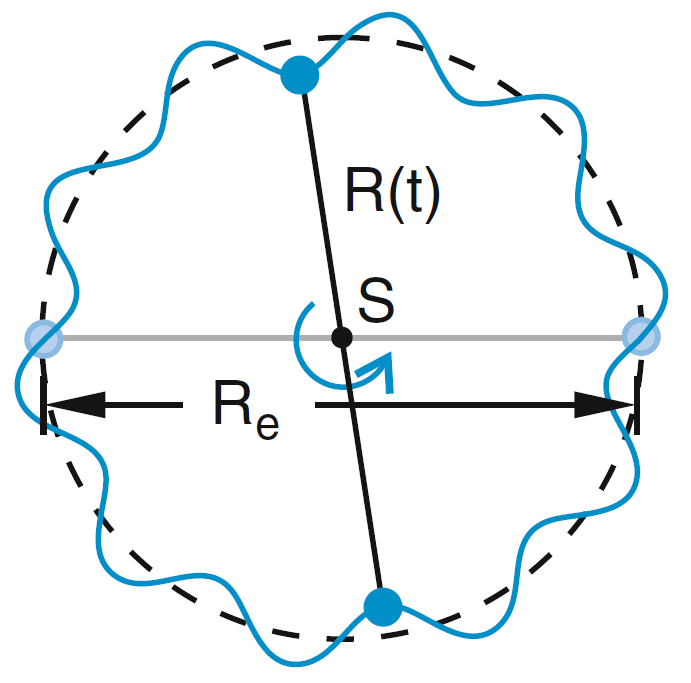
\includegraphics[width=.35\textwidth]{Q20/images/VibratingRotor.PNG}
    \caption{Vibrerende rotor.}
    \label{fig:Q20_VibratingRotor}
\end{figure}

På \cref{fig:Q20_VibratingRotor} kan det ses, at den vibrationelle frekvens er større end den rotationelle frekvens med én eller to størrelsesordener; molekylet vibrerer altså typisk 5-100 gange under én rotation. Dog, hvis man kigger på det, så vil hver vibrationelle tilstand have mange mulige rotationer tilknyttet, hvilket kan ses på \cref{fig:Q20_VibrationOgRotationPotential}.

\begin{figure}[!h]
    \centering
    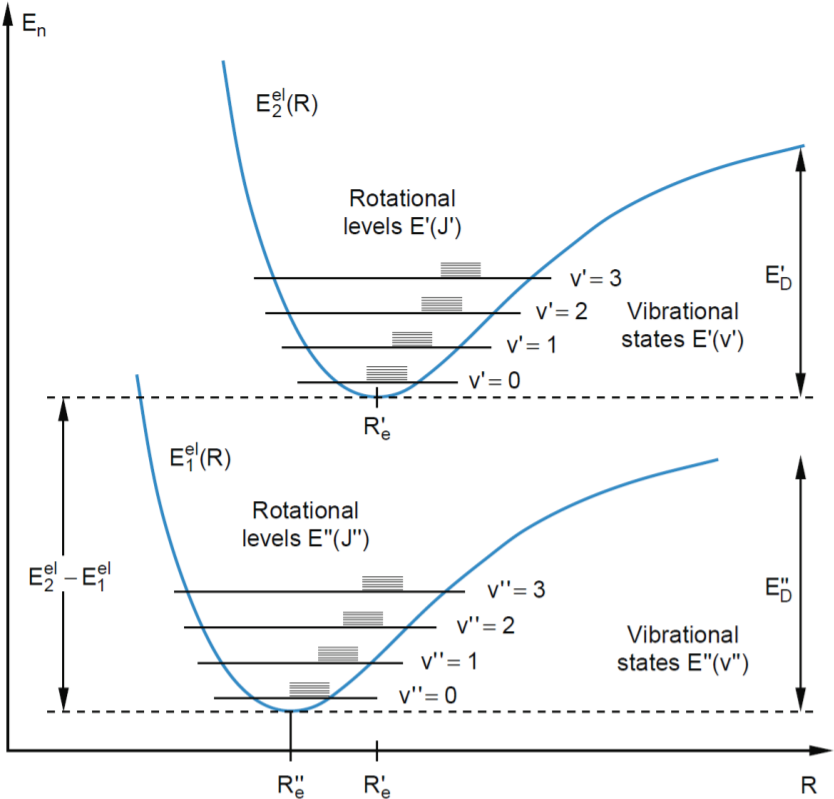
\includegraphics[width=.8\textwidth]{Q20/images/VibrationOgRotationIPotentialDiatomartMolekyle.PNG}
    \caption{Rotationelle og vibrationelle tilstande for et diatomart molekyle i to forskellige elektrontilstande.}
    \label{fig:Q20_VibrationOgRotationPotential}
\end{figure}



\end{document}

%%%%%%%%%%%%%%%%%%%%%%%%%%%%%%%%%%%%%%%%%%%%%%%%%%%%%%%%%%%%%%%%%%%%%%%%%%